% Options for packages loaded elsewhere
\PassOptionsToPackage{unicode}{hyperref}
\PassOptionsToPackage{hyphens}{url}
\PassOptionsToPackage{dvipsnames,svgnames,x11names}{xcolor}
%
\documentclass[
  letterpaper,
  DIV=11,
  numbers=noendperiod]{scrartcl}

\usepackage{amsmath,amssymb}
\usepackage{iftex}
\ifPDFTeX
  \usepackage[T1]{fontenc}
  \usepackage[utf8]{inputenc}
  \usepackage{textcomp} % provide euro and other symbols
\else % if luatex or xetex
  \usepackage{unicode-math}
  \defaultfontfeatures{Scale=MatchLowercase}
  \defaultfontfeatures[\rmfamily]{Ligatures=TeX,Scale=1}
\fi
\usepackage{lmodern}
\ifPDFTeX\else  
    % xetex/luatex font selection
\fi
% Use upquote if available, for straight quotes in verbatim environments
\IfFileExists{upquote.sty}{\usepackage{upquote}}{}
\IfFileExists{microtype.sty}{% use microtype if available
  \usepackage[]{microtype}
  \UseMicrotypeSet[protrusion]{basicmath} % disable protrusion for tt fonts
}{}
\makeatletter
\@ifundefined{KOMAClassName}{% if non-KOMA class
  \IfFileExists{parskip.sty}{%
    \usepackage{parskip}
  }{% else
    \setlength{\parindent}{0pt}
    \setlength{\parskip}{6pt plus 2pt minus 1pt}}
}{% if KOMA class
  \KOMAoptions{parskip=half}}
\makeatother
\usepackage{xcolor}
\setlength{\emergencystretch}{3em} % prevent overfull lines
\setcounter{secnumdepth}{-\maxdimen} % remove section numbering
% Make \paragraph and \subparagraph free-standing
\makeatletter
\ifx\paragraph\undefined\else
  \let\oldparagraph\paragraph
  \renewcommand{\paragraph}{
    \@ifstar
      \xxxParagraphStar
      \xxxParagraphNoStar
  }
  \newcommand{\xxxParagraphStar}[1]{\oldparagraph*{#1}\mbox{}}
  \newcommand{\xxxParagraphNoStar}[1]{\oldparagraph{#1}\mbox{}}
\fi
\ifx\subparagraph\undefined\else
  \let\oldsubparagraph\subparagraph
  \renewcommand{\subparagraph}{
    \@ifstar
      \xxxSubParagraphStar
      \xxxSubParagraphNoStar
  }
  \newcommand{\xxxSubParagraphStar}[1]{\oldsubparagraph*{#1}\mbox{}}
  \newcommand{\xxxSubParagraphNoStar}[1]{\oldsubparagraph{#1}\mbox{}}
\fi
\makeatother

\usepackage{color}
\usepackage{fancyvrb}
\newcommand{\VerbBar}{|}
\newcommand{\VERB}{\Verb[commandchars=\\\{\}]}
\DefineVerbatimEnvironment{Highlighting}{Verbatim}{commandchars=\\\{\}}
% Add ',fontsize=\small' for more characters per line
\usepackage{framed}
\definecolor{shadecolor}{RGB}{241,243,245}
\newenvironment{Shaded}{\begin{snugshade}}{\end{snugshade}}
\newcommand{\AlertTok}[1]{\textcolor[rgb]{0.68,0.00,0.00}{#1}}
\newcommand{\AnnotationTok}[1]{\textcolor[rgb]{0.37,0.37,0.37}{#1}}
\newcommand{\AttributeTok}[1]{\textcolor[rgb]{0.40,0.45,0.13}{#1}}
\newcommand{\BaseNTok}[1]{\textcolor[rgb]{0.68,0.00,0.00}{#1}}
\newcommand{\BuiltInTok}[1]{\textcolor[rgb]{0.00,0.23,0.31}{#1}}
\newcommand{\CharTok}[1]{\textcolor[rgb]{0.13,0.47,0.30}{#1}}
\newcommand{\CommentTok}[1]{\textcolor[rgb]{0.37,0.37,0.37}{#1}}
\newcommand{\CommentVarTok}[1]{\textcolor[rgb]{0.37,0.37,0.37}{\textit{#1}}}
\newcommand{\ConstantTok}[1]{\textcolor[rgb]{0.56,0.35,0.01}{#1}}
\newcommand{\ControlFlowTok}[1]{\textcolor[rgb]{0.00,0.23,0.31}{\textbf{#1}}}
\newcommand{\DataTypeTok}[1]{\textcolor[rgb]{0.68,0.00,0.00}{#1}}
\newcommand{\DecValTok}[1]{\textcolor[rgb]{0.68,0.00,0.00}{#1}}
\newcommand{\DocumentationTok}[1]{\textcolor[rgb]{0.37,0.37,0.37}{\textit{#1}}}
\newcommand{\ErrorTok}[1]{\textcolor[rgb]{0.68,0.00,0.00}{#1}}
\newcommand{\ExtensionTok}[1]{\textcolor[rgb]{0.00,0.23,0.31}{#1}}
\newcommand{\FloatTok}[1]{\textcolor[rgb]{0.68,0.00,0.00}{#1}}
\newcommand{\FunctionTok}[1]{\textcolor[rgb]{0.28,0.35,0.67}{#1}}
\newcommand{\ImportTok}[1]{\textcolor[rgb]{0.00,0.46,0.62}{#1}}
\newcommand{\InformationTok}[1]{\textcolor[rgb]{0.37,0.37,0.37}{#1}}
\newcommand{\KeywordTok}[1]{\textcolor[rgb]{0.00,0.23,0.31}{\textbf{#1}}}
\newcommand{\NormalTok}[1]{\textcolor[rgb]{0.00,0.23,0.31}{#1}}
\newcommand{\OperatorTok}[1]{\textcolor[rgb]{0.37,0.37,0.37}{#1}}
\newcommand{\OtherTok}[1]{\textcolor[rgb]{0.00,0.23,0.31}{#1}}
\newcommand{\PreprocessorTok}[1]{\textcolor[rgb]{0.68,0.00,0.00}{#1}}
\newcommand{\RegionMarkerTok}[1]{\textcolor[rgb]{0.00,0.23,0.31}{#1}}
\newcommand{\SpecialCharTok}[1]{\textcolor[rgb]{0.37,0.37,0.37}{#1}}
\newcommand{\SpecialStringTok}[1]{\textcolor[rgb]{0.13,0.47,0.30}{#1}}
\newcommand{\StringTok}[1]{\textcolor[rgb]{0.13,0.47,0.30}{#1}}
\newcommand{\VariableTok}[1]{\textcolor[rgb]{0.07,0.07,0.07}{#1}}
\newcommand{\VerbatimStringTok}[1]{\textcolor[rgb]{0.13,0.47,0.30}{#1}}
\newcommand{\WarningTok}[1]{\textcolor[rgb]{0.37,0.37,0.37}{\textit{#1}}}

\providecommand{\tightlist}{%
  \setlength{\itemsep}{0pt}\setlength{\parskip}{0pt}}\usepackage{longtable,booktabs,array}
\usepackage{calc} % for calculating minipage widths
% Correct order of tables after \paragraph or \subparagraph
\usepackage{etoolbox}
\makeatletter
\patchcmd\longtable{\par}{\if@noskipsec\mbox{}\fi\par}{}{}
\makeatother
% Allow footnotes in longtable head/foot
\IfFileExists{footnotehyper.sty}{\usepackage{footnotehyper}}{\usepackage{footnote}}
\makesavenoteenv{longtable}
\usepackage{graphicx}
\makeatletter
\def\maxwidth{\ifdim\Gin@nat@width>\linewidth\linewidth\else\Gin@nat@width\fi}
\def\maxheight{\ifdim\Gin@nat@height>\textheight\textheight\else\Gin@nat@height\fi}
\makeatother
% Scale images if necessary, so that they will not overflow the page
% margins by default, and it is still possible to overwrite the defaults
% using explicit options in \includegraphics[width, height, ...]{}
\setkeys{Gin}{width=\maxwidth,height=\maxheight,keepaspectratio}
% Set default figure placement to htbp
\makeatletter
\def\fps@figure{htbp}
\makeatother

\usepackage{fvextra}
\DefineVerbatimEnvironment{Highlighting}{Verbatim}{breaklines,commandchars=\\\{\}}
\KOMAoption{captions}{tableheading}
\makeatletter
\@ifpackageloaded{caption}{}{\usepackage{caption}}
\AtBeginDocument{%
\ifdefined\contentsname
  \renewcommand*\contentsname{Table of contents}
\else
  \newcommand\contentsname{Table of contents}
\fi
\ifdefined\listfigurename
  \renewcommand*\listfigurename{List of Figures}
\else
  \newcommand\listfigurename{List of Figures}
\fi
\ifdefined\listtablename
  \renewcommand*\listtablename{List of Tables}
\else
  \newcommand\listtablename{List of Tables}
\fi
\ifdefined\figurename
  \renewcommand*\figurename{Figure}
\else
  \newcommand\figurename{Figure}
\fi
\ifdefined\tablename
  \renewcommand*\tablename{Table}
\else
  \newcommand\tablename{Table}
\fi
}
\@ifpackageloaded{float}{}{\usepackage{float}}
\floatstyle{ruled}
\@ifundefined{c@chapter}{\newfloat{codelisting}{h}{lop}}{\newfloat{codelisting}{h}{lop}[chapter]}
\floatname{codelisting}{Listing}
\newcommand*\listoflistings{\listof{codelisting}{List of Listings}}
\makeatother
\makeatletter
\makeatother
\makeatletter
\@ifpackageloaded{caption}{}{\usepackage{caption}}
\@ifpackageloaded{subcaption}{}{\usepackage{subcaption}}
\makeatother

\ifLuaTeX
  \usepackage{selnolig}  % disable illegal ligatures
\fi
\usepackage{bookmark}

\IfFileExists{xurl.sty}{\usepackage{xurl}}{} % add URL line breaks if available
\urlstyle{same} % disable monospaced font for URLs
\hypersetup{
  pdftitle={ps4},
  colorlinks=true,
  linkcolor={blue},
  filecolor={Maroon},
  citecolor={Blue},
  urlcolor={Blue},
  pdfcreator={LaTeX via pandoc}}


\title{ps4}
\author{}
\date{}

\begin{document}
\maketitle

\RecustomVerbatimEnvironment{verbatim}{Verbatim}{
  showspaces = false,
  showtabs = false,
  breaksymbolleft={},
  breaklines
}


\textbf{PS4:} Due Sat Nov 2 at 5:00PM Central. Worth 100 points. \#\#\#
Academic integrity statement We checked Googled commands/ways to go
about getting the output needed. I have included the links where I
learned from. Additionally, I used ChatGPT for help with debugging
double checking the flow of my code. I also referred to code from last
quarter's python class for grouping, datetime, dictionary, length,
float, round, print,a nd reset index functinos. ALso checked
https://stackoverflow.com/questions/tagged/geospatial for specific
codign questions.

\begin{enumerate}
\def\labelenumi{\arabic{enumi}.}
\tightlist
\item
  ``This submission is my work alone and complies with the 30538
  integrity policy.'' \textbf{CT} \textbf{EA}
\item
  ``I have uploaded the names of anyone I worked with on the problem set
  \textbf{\href{https://docs.google.com/forms/d/1-zzHx762odGlpVWtgdIC55vqF-j3gqdAp6Pno1rIGK0/edit}{here}}''
  **\_\_** (1 point)
\item
  Late coins used this pset: \textbf{3} Late coins left after
  submission: \textbf{1}
\end{enumerate}

\subsection{Style Points (10 pts)}\label{style-points-10-pts}

\subsection{Submission Steps (10 pts)}\label{submission-steps-10-pts}

\begin{enumerate}
\def\labelenumi{\arabic{enumi}.}
\tightlist
\item
  This problem set is a paired problem set.
\item
  Play paper, scissors, rock to determine who goes first. Call that
  person \emph{Partner 1}.

  \begin{itemize}
  \tightlist
  \item
    Partner 1 (cmtee):
  \item
    Partner 2 (eandujar):
  \end{itemize}
\item
  ``This submission is our work alone and complies with the 30538
  integrity policy.'' Add your initials to indicate your agreement:
  **\_\_** **\_\_**
\item
  ``I have uploaded the names of anyone else other than my partner and I
  worked with on the problem set
  \textbf{\href{https://docs.google.com/forms/d/185usrCREQaUbvAXpWhChkjghdGgmAZXA3lPWpXLLsts/edit}{here}}''
  (1 point)
\item
  Late coins used this pset: **\textbackslash3** Late coins left after
  submission: **\textbackslash1** \#\# Download and explore the Provider
  of Services (POS) file (10 pts)
\end{enumerate}

\begin{Shaded}
\begin{Highlighting}[]
\ImportTok{import}\NormalTok{ pandas }\ImportTok{as}\NormalTok{ pd}
\ImportTok{import}\NormalTok{ os}
\ImportTok{import}\NormalTok{ matplotlib.pyplot }\ImportTok{as}\NormalTok{ plt}
\ImportTok{import}\NormalTok{ geopandas }\ImportTok{as}\NormalTok{ gpd}
\ImportTok{import}\NormalTok{ time}
\end{Highlighting}
\end{Shaded}

\begin{enumerate}
\def\labelenumi{\arabic{enumi}.}
\tightlist
\item
  I pulled
\end{enumerate}

FAC\_NAME STATE\_CD PRVDR\_CTGRY\_CD PRVDR\_CTGRY\_SBTYP\_CD ZIP-CD
PGM\_TRMNTN\_CD PGM\_TRMNTN\_CD 2.

\begin{Shaded}
\begin{Highlighting}[]
\CommentTok{\# Load the 2016 dataset}
\NormalTok{df }\OperatorTok{=}\NormalTok{ pd.read\_csv(}
    \StringTok{\textquotesingle{}C:/Users/clari/OneDrive/Documents/Python II/pos\_files/pos2016.csv\textquotesingle{}}\NormalTok{)}
\CommentTok{\# change the path as needed}
\end{Highlighting}
\end{Shaded}

\begin{Shaded}
\begin{Highlighting}[]
\CommentTok{\# Filter for short{-}term hospitals (provider type code 01 and subtype code 01)}
\NormalTok{st\_hospitals\_2016 }\OperatorTok{=}\NormalTok{ df[(df[}\StringTok{\textquotesingle{}PRVDR\_CTGRY\_CD\textquotesingle{}}\NormalTok{] }\OperatorTok{==} \DecValTok{1}\NormalTok{) }\OperatorTok{\&}
\NormalTok{                       (df[}\StringTok{\textquotesingle{}PRVDR\_CTGRY\_SBTYP\_CD\textquotesingle{}}\NormalTok{] }\OperatorTok{==} \DecValTok{1}\NormalTok{)]}
\BuiltInTok{print}\NormalTok{(}\BuiltInTok{len}\NormalTok{(st\_hospitals\_2016))}
\end{Highlighting}
\end{Shaded}

\begin{verbatim}
7245
\end{verbatim}

\begin{verbatim}
a.There are 7,245 reported in this data.This number doesn't make sense because there seem to be too many short-term hospitals.
b. According to AHA, there were only 4,840 in 2016, so this number doesn't make sense. This could be due to differences in
 definitions, inclusion criteria, and scope. Maybe this raw dataset  has a broader range of facilities certified for Medicare/Medicaid billing, which increases the cout. Maybe the includsion of subtypes increased our count too.
\end{verbatim}

https://www.aha.org/system/files/2018-02/2018-aha-hospital-fast-facts\_0.pdf

\begin{enumerate}
\def\labelenumi{\arabic{enumi}.}
\setcounter{enumi}{2}
\tightlist
\item
\end{enumerate}

\begin{Shaded}
\begin{Highlighting}[]
\CommentTok{\# Define the path to your folder containing the POS files}
\NormalTok{folder\_path }\OperatorTok{=} \VerbatimStringTok{r\textquotesingle{}C:/Users/clari/OneDrive/Documents/Python II/pos\_files\textquotesingle{}}
\CommentTok{\# path for eddie: r\textquotesingle{}C:\textbackslash{}Users\textbackslash{}eddie\textbackslash{}Downloads\textbackslash{}pos2016.csv\textquotesingle{}}

\CommentTok{\# List all files in the directory to check if they exist}
\BuiltInTok{print}\NormalTok{(}\StringTok{"Files in directory:"}\NormalTok{)}
\ControlFlowTok{for} \BuiltInTok{file} \KeywordTok{in}\NormalTok{ os.listdir(folder\_path):}
    \BuiltInTok{print}\NormalTok{(}\BuiltInTok{file}\NormalTok{)}

\CommentTok{\# Define a function to load CSV files with different encodings and filter for short{-}term hospitals}
\KeywordTok{def}\NormalTok{ load\_and\_filter\_csv(file\_name, encodings, year):}
    \ControlFlowTok{for}\NormalTok{ encoding }\KeywordTok{in}\NormalTok{ encodings:}
        \ControlFlowTok{try}\NormalTok{:}
            \CommentTok{\# Try reading the file with a specified encoding}
\NormalTok{            df }\OperatorTok{=}\NormalTok{ pd.read\_csv(os.path.join(folder\_path, file\_name),}
\NormalTok{                             encoding}\OperatorTok{=}\NormalTok{encoding, engine}\OperatorTok{=}\StringTok{\textquotesingle{}python\textquotesingle{}}\NormalTok{)}
            \BuiltInTok{print}\NormalTok{(}\SpecialStringTok{f\textquotesingle{}Successfully loaded }\SpecialCharTok{\{}\NormalTok{file\_name}\SpecialCharTok{\}}\SpecialStringTok{ with encoding }\SpecialCharTok{\{}\NormalTok{encoding}\SpecialCharTok{\}}\SpecialStringTok{.\textquotesingle{}}\NormalTok{)}

            \CommentTok{\# Filter for short{-}term hospitals (provider type code 01 and subtype code 01)}
\NormalTok{            st\_hospitals }\OperatorTok{=}\NormalTok{ df[(df[}\StringTok{\textquotesingle{}PRVDR\_CTGRY\_CD\textquotesingle{}}\NormalTok{] }\OperatorTok{==} \DecValTok{1}\NormalTok{) }\OperatorTok{\&}
\NormalTok{                              (df[}\StringTok{\textquotesingle{}PRVDR\_CTGRY\_SBTYP\_CD\textquotesingle{}}\NormalTok{] }\OperatorTok{==} \DecValTok{1}\NormalTok{)]}
            \CommentTok{\# Add a \textquotesingle{}Year\textquotesingle{} column to the DataFrame}
\NormalTok{            st\_hospitals[}\StringTok{\textquotesingle{}Year\textquotesingle{}}\NormalTok{] }\OperatorTok{=}\NormalTok{ year}

            \ControlFlowTok{return}\NormalTok{ st\_hospitals  }\CommentTok{\# Return the filtered DataFrame if loaded successfully}
        \ControlFlowTok{except} \PreprocessorTok{Exception} \ImportTok{as}\NormalTok{ e:}
            \BuiltInTok{print}\NormalTok{(}\SpecialStringTok{f\textquotesingle{}Error loading }\SpecialCharTok{\{}\NormalTok{file\_name}\SpecialCharTok{\}}\SpecialStringTok{ with encoding }\SpecialCharTok{\{}\NormalTok{encoding}\SpecialCharTok{\}}\SpecialStringTok{: }\SpecialCharTok{\{}\NormalTok{e}\SpecialCharTok{\}}\SpecialStringTok{\textquotesingle{}}\NormalTok{)}
    \ControlFlowTok{return} \VariableTok{None}  \CommentTok{\# Return None if all attempts fail}


\CommentTok{\# List of encodings to try}
\NormalTok{encodings }\OperatorTok{=}\NormalTok{ [}\StringTok{\textquotesingle{}utf{-}8\textquotesingle{}}\NormalTok{, }\StringTok{\textquotesingle{}ISO{-}8859{-}1\textquotesingle{}}\NormalTok{, }\StringTok{\textquotesingle{}latin1\textquotesingle{}}\NormalTok{, }\StringTok{\textquotesingle{}utf{-}8{-}sig\textquotesingle{}}\NormalTok{, }\StringTok{\textquotesingle{}cp1252\textquotesingle{}}\NormalTok{]}

\CommentTok{\# List of file names and corresponding years}
\NormalTok{files\_with\_years }\OperatorTok{=}\NormalTok{ [(}\StringTok{\textquotesingle{}pos2016.csv\textquotesingle{}}\NormalTok{, }\DecValTok{2016}\NormalTok{), (}\StringTok{\textquotesingle{}pos2017.csv\textquotesingle{}}\NormalTok{, }\DecValTok{2017}\NormalTok{),}
\NormalTok{                    (}\StringTok{\textquotesingle{}pos2018.csv\textquotesingle{}}\NormalTok{, }\DecValTok{2018}\NormalTok{), (}\StringTok{\textquotesingle{}pos2019.csv\textquotesingle{}}\NormalTok{, }\DecValTok{2019}\NormalTok{)]}

\CommentTok{\# Load datasets for all years and filter for short{-}term hospitals}
\NormalTok{appended\_dfs }\OperatorTok{=}\NormalTok{ []}
\ControlFlowTok{for}\NormalTok{ file\_name, year }\KeywordTok{in}\NormalTok{ files\_with\_years:}
\NormalTok{    df }\OperatorTok{=}\NormalTok{ load\_and\_filter\_csv(file\_name, encodings, year)}
    \ControlFlowTok{if}\NormalTok{ df }\KeywordTok{is} \KeywordTok{not} \VariableTok{None}\NormalTok{:}
\NormalTok{        appended\_dfs.append(df)}

\CommentTok{\# Check if we successfully loaded and filtered data for all years}
\ControlFlowTok{if} \BuiltInTok{len}\NormalTok{(appended\_dfs) }\OperatorTok{==} \BuiltInTok{len}\NormalTok{(files\_with\_years):}
    \CommentTok{\# Append all filtered DataFrames together into one DataFrame}
\NormalTok{    combined\_df }\OperatorTok{=}\NormalTok{ pd.concat(appended\_dfs, ignore\_index}\OperatorTok{=}\VariableTok{True}\NormalTok{)}
    \BuiltInTok{print}\NormalTok{(}\StringTok{"Successfully appended all datasets."}\NormalTok{)}

    \CommentTok{\# Save the combined DataFrame to a CSV file named \textquotesingle{}pos\_6789.csv\textquotesingle{}}
\NormalTok{    output\_file }\OperatorTok{=}\NormalTok{ os.path.join(folder\_path, }\StringTok{\textquotesingle{}pos\_6789.csv\textquotesingle{}}\NormalTok{)}
\NormalTok{    combined\_df.to\_csv(output\_file, index}\OperatorTok{=}\VariableTok{False}\NormalTok{)}
    \BuiltInTok{print}\NormalTok{(}\SpecialStringTok{f"Combined dataset saved as }\SpecialCharTok{\{}\NormalTok{output\_file}\SpecialCharTok{\}}\SpecialStringTok{"}\NormalTok{)}
\ControlFlowTok{else}\NormalTok{:}
    \BuiltInTok{print}\NormalTok{(}\StringTok{"Some files could not be loaded or filtered."}\NormalTok{)}

\CommentTok{\# Optionally, print the first few rows of the combined DataFrame to verify}
\ControlFlowTok{if} \BuiltInTok{len}\NormalTok{(appended\_dfs) }\OperatorTok{\textgreater{}} \DecValTok{0}\NormalTok{:}
    \BuiltInTok{print}\NormalTok{(combined\_df.head())}
\end{Highlighting}
\end{Shaded}

\begin{verbatim}
Files in directory:
corrected_suspected_hospital_closures_2016_2018.csv
corrected_suspected_hospital_closures_2016_2019.csv
pos2016.csv
pos2017.csv
pos2018.csv
pos2019.csv
pos_6789.csv
suspected_hospital_closures_2016_2019_sorted.csv
suspected_short_term_hospital_closures_2016_2019.csv
suspected_short_term_hospital_closures_2016_2019_sorted.csv
tx_closures_by_zip.csv
Successfully loaded pos2016.csv with encoding utf-8.
\end{verbatim}

\begin{verbatim}
C:\Users\clari\AppData\Local\Temp\ipykernel_9008\3845987685.py:23: SettingWithCopyWarning:


A value is trying to be set on a copy of a slice from a DataFrame.
Try using .loc[row_indexer,col_indexer] = value instead

See the caveats in the documentation: https://pandas.pydata.org/pandas-docs/stable/user_guide/indexing.html#returning-a-view-versus-a-copy
\end{verbatim}

\begin{verbatim}
Successfully loaded pos2017.csv with encoding utf-8.
Error loading pos2018.csv with encoding utf-8: 'utf-8' codec can't decode byte 0xa0 in position 7482: invalid start byte
\end{verbatim}

\begin{verbatim}
C:\Users\clari\AppData\Local\Temp\ipykernel_9008\3845987685.py:23: SettingWithCopyWarning:


A value is trying to be set on a copy of a slice from a DataFrame.
Try using .loc[row_indexer,col_indexer] = value instead

See the caveats in the documentation: https://pandas.pydata.org/pandas-docs/stable/user_guide/indexing.html#returning-a-view-versus-a-copy
\end{verbatim}

\begin{verbatim}
Successfully loaded pos2018.csv with encoding ISO-8859-1.
Error loading pos2019.csv with encoding utf-8: 'utf-8' codec can't decode byte 0x98 in position 4114: invalid start byte
\end{verbatim}

\begin{verbatim}
C:\Users\clari\AppData\Local\Temp\ipykernel_9008\3845987685.py:23: SettingWithCopyWarning:


A value is trying to be set on a copy of a slice from a DataFrame.
Try using .loc[row_indexer,col_indexer] = value instead

See the caveats in the documentation: https://pandas.pydata.org/pandas-docs/stable/user_guide/indexing.html#returning-a-view-versus-a-copy
\end{verbatim}

\begin{verbatim}
Successfully loaded pos2019.csv with encoding ISO-8859-1.
Successfully appended all datasets.
Combined dataset saved as C:/Users/clari/OneDrive/Documents/Python II/pos_files\pos_6789.csv
   PRVDR_CTGRY_SBTYP_CD  PRVDR_CTGRY_CD                          FAC_NAME  \
0                   1.0               1  SOUTHEAST ALABAMA MEDICAL CENTER   
1                   1.0               1            NORTH JACKSON HOSPITAL   
2                   1.0               1     MARSHALL MEDICAL CENTER SOUTH   
3                   1.0               1    ELIZA COFFEE MEMORIAL HOSPITAL   
4                   1.0               1          MIZELL MEMORIAL HOSPITAL   

  PRVDR_NUM STATE_CD   ZIP_CD  GNRL_FAC_TYPE_CD  PGM_TRMNTN_CD  Year  
0    010001       AL  36301.0               1.0              0  2016  
1    010004       AL  35740.0               1.0              1  2016  
2    010005       AL  35957.0               1.0              0  2016  
3    010006       AL  35631.0               1.0              0  2016  
4    010007       AL  36467.0               1.0              0  2016  
\end{verbatim}

\begin{verbatim}
C:\Users\clari\AppData\Local\Temp\ipykernel_9008\3845987685.py:23: SettingWithCopyWarning:


A value is trying to be set on a copy of a slice from a DataFrame.
Try using .loc[row_indexer,col_indexer] = value instead

See the caveats in the documentation: https://pandas.pydata.org/pandas-docs/stable/user_guide/indexing.html#returning-a-view-versus-a-copy
\end{verbatim}

There was a utf-8 error, so I asked chatGPT how to fix it

\begin{Shaded}
\begin{Highlighting}[]
\NormalTok{combined\_df }\OperatorTok{=}\NormalTok{ pd.read\_csv(os.path.join(folder\_path, }\StringTok{\textquotesingle{}pos\_6789.csv\textquotesingle{}}\NormalTok{))}

\CommentTok{\# Group by \textquotesingle{}Year\textquotesingle{} and count the number of rows per year}
\NormalTok{hospitals\_by\_year }\OperatorTok{=}\NormalTok{ combined\_df.groupby(}\StringTok{\textquotesingle{}Year\textquotesingle{}}\NormalTok{).size()}

\CommentTok{\# Plotting the number of hospitals by year}
\NormalTok{plt.figure(figsize}\OperatorTok{=}\NormalTok{(}\DecValTok{8}\NormalTok{, }\DecValTok{5}\NormalTok{))}
\NormalTok{hospitals\_by\_year.plot(kind}\OperatorTok{=}\StringTok{\textquotesingle{}bar\textquotesingle{}}\NormalTok{, color}\OperatorTok{=}\StringTok{\textquotesingle{}lightcoral\textquotesingle{}}\NormalTok{)}
\NormalTok{plt.title(}\StringTok{\textquotesingle{}Number of Hospitals by Year\textquotesingle{}}\NormalTok{)}
\NormalTok{plt.xlabel(}\StringTok{\textquotesingle{}Year\textquotesingle{}}\NormalTok{)}
\NormalTok{plt.ylabel(}\StringTok{\textquotesingle{}Number of Hospitals\textquotesingle{}}\NormalTok{)}
\NormalTok{plt.xticks(rotation}\OperatorTok{=}\DecValTok{0}\NormalTok{)}
\NormalTok{plt.show()}
\end{Highlighting}
\end{Shaded}

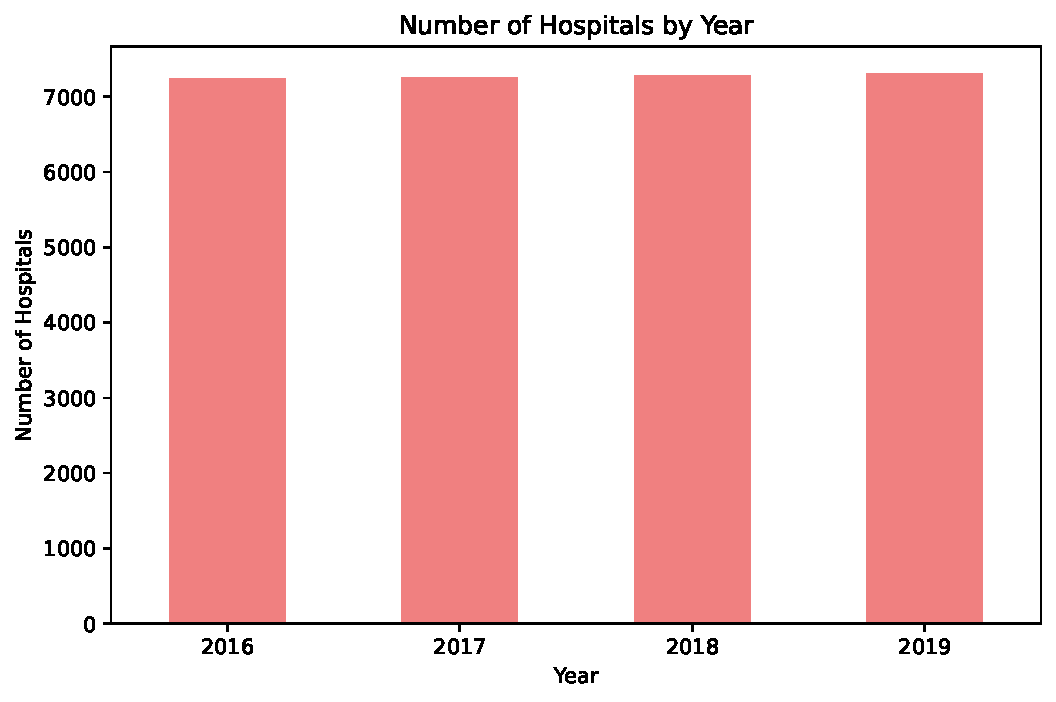
\includegraphics{pset4_ANSWERS_files/figure-pdf/cell-6-output-1.pdf}

\begin{enumerate}
\def\labelenumi{\arabic{enumi}.}
\setcounter{enumi}{3}
\tightlist
\item
  \begin{enumerate}
  \def\labelenumii{\alph{enumii}.}
  \tightlist
  \item
  \end{enumerate}
\end{enumerate}

\begin{Shaded}
\begin{Highlighting}[]
\NormalTok{unique\_hospitals\_by\_year }\OperatorTok{=}\NormalTok{ combined\_df.groupby(}\StringTok{\textquotesingle{}Year\textquotesingle{}}\NormalTok{)[}\StringTok{\textquotesingle{}PRVDR\_NUM\textquotesingle{}}\NormalTok{].nunique()}

\CommentTok{\# Plotting the number of unique hospitals by year}
\NormalTok{plt.figure(figsize}\OperatorTok{=}\NormalTok{(}\DecValTok{8}\NormalTok{, }\DecValTok{5}\NormalTok{))}
\NormalTok{unique\_hospitals\_by\_year.plot(kind}\OperatorTok{=}\StringTok{\textquotesingle{}bar\textquotesingle{}}\NormalTok{, color}\OperatorTok{=}\StringTok{\textquotesingle{}lightcoral\textquotesingle{}}\NormalTok{, edgecolor}\OperatorTok{=}\StringTok{\textquotesingle{}black\textquotesingle{}}\NormalTok{)}
\NormalTok{plt.title(}\StringTok{\textquotesingle{}Number of Unique Hospitals by Year\textquotesingle{}}\NormalTok{, fontsize}\OperatorTok{=}\DecValTok{16}\NormalTok{)}
\NormalTok{plt.xlabel(}\StringTok{\textquotesingle{}Year\textquotesingle{}}\NormalTok{, fontsize}\OperatorTok{=}\DecValTok{14}\NormalTok{)}
\NormalTok{plt.ylabel(}\StringTok{\textquotesingle{}Number of Unique Hospitals\textquotesingle{}}\NormalTok{, fontsize}\OperatorTok{=}\DecValTok{14}\NormalTok{)}
\NormalTok{plt.xticks(rotation}\OperatorTok{=}\DecValTok{0}\NormalTok{)}
\NormalTok{plt.grid(axis}\OperatorTok{=}\StringTok{\textquotesingle{}y\textquotesingle{}}\NormalTok{, linestyle}\OperatorTok{=}\StringTok{\textquotesingle{}{-}{-}\textquotesingle{}}\NormalTok{, alpha}\OperatorTok{=}\FloatTok{0.7}\NormalTok{)}
\NormalTok{plt.tight\_layout()}
\NormalTok{plt.show()}
\end{Highlighting}
\end{Shaded}

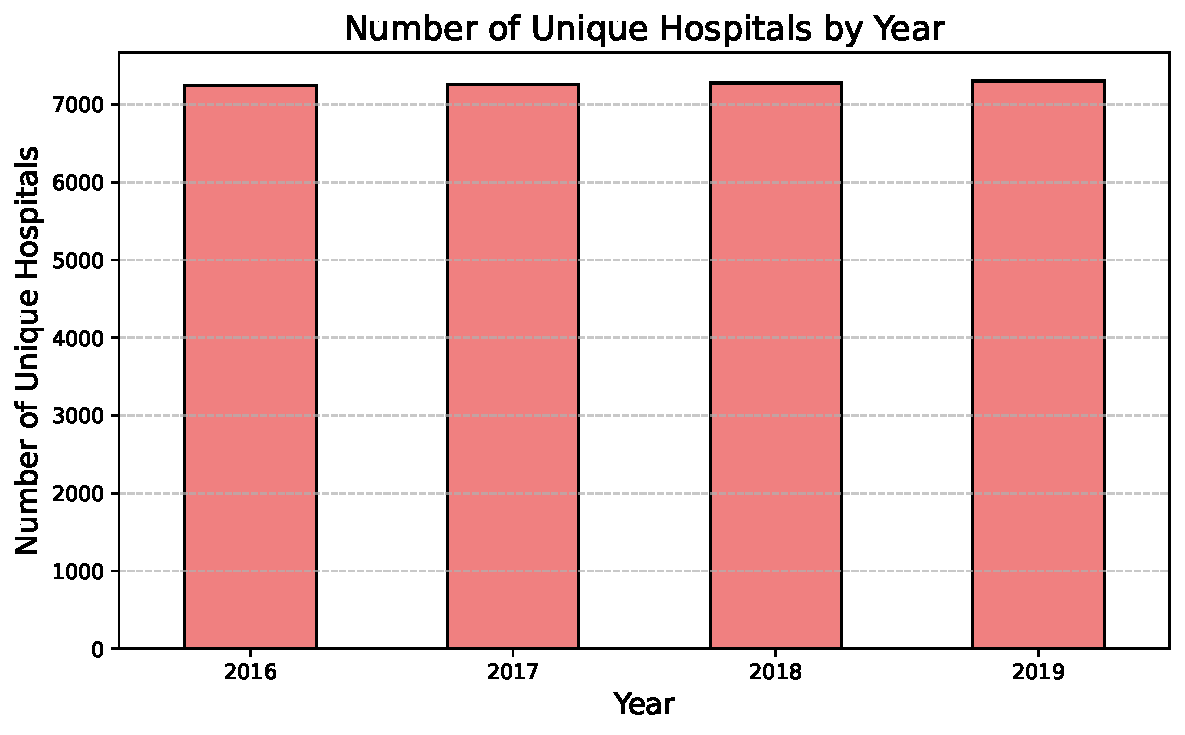
\includegraphics{pset4_ANSWERS_files/figure-pdf/cell-7-output-1.pdf}

\begin{verbatim}
b.Both plots (total vs. unique hospitals) give the same result. This strongly suggests that the  dataset is clean and well-structured, with no duplicate entries for hospitals based on their CMS certification numbers (PRVDR_NUM). Each hospital appears only once per year, which means I can confidently proceed with further analysis without worrying about duplicate data affecting your results.
\end{verbatim}

\subsection{Identify hospital closures in POS file (15 pts)
(*)}\label{identify-hospital-closures-in-pos-file-15-pts}

\begin{Shaded}
\begin{Highlighting}[]
\ImportTok{import}\NormalTok{ altair }\ImportTok{as}\NormalTok{ alt}
\NormalTok{alt.renderers.enable(}\StringTok{"png"}\NormalTok{)}
\ImportTok{from}\NormalTok{ vega\_datasets }\ImportTok{import}\NormalTok{ data }\ImportTok{as}\NormalTok{ vega\_data}
\ImportTok{import}\NormalTok{ warnings }
\NormalTok{warnings.filterwarnings(}\StringTok{\textquotesingle{}ignore\textquotesingle{}}\NormalTok{)}

\NormalTok{folder\_path }\OperatorTok{=} \VerbatimStringTok{r\textquotesingle{}C:/Users/clari/OneDrive/Documents/Python II/pos\_files/pos\_6789.csv\textquotesingle{}}
\CommentTok{\# path for eddie: \textquotesingle{}C:\textbackslash{}Users\textbackslash{}eddie\textbackslash{}Downloads\textbackslash{}pos\_6789 (2).csv\textquotesingle{}}

\NormalTok{df }\OperatorTok{=}\NormalTok{ pd.read\_csv(folder\_path)}
\end{Highlighting}
\end{Shaded}

2.1

Checking columns to verify

\begin{Shaded}
\begin{Highlighting}[]
\CommentTok{\# Get a list of all column names}
\NormalTok{column\_names }\OperatorTok{=}\NormalTok{ df.columns.tolist()}

\CommentTok{\# Print the list of column names}
\BuiltInTok{print}\NormalTok{(column\_names)}
\end{Highlighting}
\end{Shaded}

\begin{verbatim}
['PRVDR_CTGRY_SBTYP_CD', 'PRVDR_CTGRY_CD', 'FAC_NAME', 'PRVDR_NUM', 'STATE_CD', 'ZIP_CD', 'GNRL_FAC_TYPE_CD', 'PGM_TRMNTN_CD', 'Year']
\end{verbatim}

\begin{Shaded}
\begin{Highlighting}[]
\CommentTok{\# Step 1: Filter hospitals active in 2016}
\NormalTok{active\_2016 }\OperatorTok{=}\NormalTok{ df[(df[}\StringTok{\textquotesingle{}Year\textquotesingle{}}\NormalTok{] }\OperatorTok{==} \DecValTok{2016}\NormalTok{) }\OperatorTok{\&}\NormalTok{ (df[}\StringTok{\textquotesingle{}PGM\_TRMNTN\_CD\textquotesingle{}}\NormalTok{] }\OperatorTok{==} \DecValTok{0}\NormalTok{)]}

\CommentTok{\# Step 2: Initialize a list to capture closures}
\NormalTok{closures }\OperatorTok{=}\NormalTok{ []}

\CommentTok{\# Step 3: Loop through each hospital that was active in 2016}
\ControlFlowTok{for}\NormalTok{ \_, row }\KeywordTok{in}\NormalTok{ active\_2016.iterrows():}
\NormalTok{    prvd\_num }\OperatorTok{=}\NormalTok{ row[}\StringTok{\textquotesingle{}PRVDR\_NUM\textquotesingle{}}\NormalTok{]}
\NormalTok{    facility\_name }\OperatorTok{=}\NormalTok{ row[}\StringTok{\textquotesingle{}FAC\_NAME\textquotesingle{}}\NormalTok{]}
\NormalTok{    zip\_code }\OperatorTok{=}\NormalTok{ row[}\StringTok{\textquotesingle{}ZIP\_CD\textquotesingle{}}\NormalTok{]}
\NormalTok{    suspected\_closure\_year }\OperatorTok{=} \VariableTok{None}

    \CommentTok{\# Check each year from 2017 to 2019}
    \ControlFlowTok{for}\NormalTok{ year }\KeywordTok{in} \BuiltInTok{range}\NormalTok{(}\DecValTok{2017}\NormalTok{, }\DecValTok{2020}\NormalTok{):}
\NormalTok{        record }\OperatorTok{=}\NormalTok{ df[(df[}\StringTok{\textquotesingle{}Year\textquotesingle{}}\NormalTok{] }\OperatorTok{==}\NormalTok{ year) }\OperatorTok{\&}\NormalTok{ (df[}\StringTok{\textquotesingle{}PRVDR\_NUM\textquotesingle{}}\NormalTok{] }\OperatorTok{==}\NormalTok{ prvd\_num)]}

        \CommentTok{\# Check if hospital is not active or missing}
        \ControlFlowTok{if}\NormalTok{ record.empty }\KeywordTok{or}\NormalTok{ record.iloc[}\DecValTok{0}\NormalTok{][}\StringTok{\textquotesingle{}PGM\_TRMNTN\_CD\textquotesingle{}}\NormalTok{] }\OperatorTok{!=} \DecValTok{0}\NormalTok{:}
\NormalTok{            suspected\_closure\_year }\OperatorTok{=}\NormalTok{ year}
            \ControlFlowTok{break}

    \CommentTok{\# If closure year was found, add it to the list}
    \ControlFlowTok{if}\NormalTok{ suspected\_closure\_year:}
\NormalTok{        closures.append(\{}
            \StringTok{\textquotesingle{}Facility Name\textquotesingle{}}\NormalTok{: facility\_name,}
            \StringTok{\textquotesingle{}ZIP\_CD\textquotesingle{}}\NormalTok{: zip\_code,}
            \StringTok{\textquotesingle{}Suspected Closure Year\textquotesingle{}}\NormalTok{: suspected\_closure\_year}
\NormalTok{        \})}

\CommentTok{\# Step 4: Convert the list to a DataFrame and display the count of closures}
\NormalTok{closures\_df }\OperatorTok{=}\NormalTok{ pd.DataFrame(closures)}
\NormalTok{closure\_count }\OperatorTok{=}\NormalTok{ closures\_df.shape[}\DecValTok{0}\NormalTok{]}

\BuiltInTok{print}\NormalTok{(}\SpecialStringTok{f"Total suspected closures: }\SpecialCharTok{\{}\NormalTok{closure\_count}\SpecialCharTok{\}}\SpecialStringTok{"}\NormalTok{)}
\NormalTok{closures\_df.head()}
\end{Highlighting}
\end{Shaded}

\begin{verbatim}
Total suspected closures: 174
\end{verbatim}

\begin{longtable}[]{@{}llll@{}}
\toprule\noalign{}
& Facility Name & ZIP\_CD & Suspected Closure Year \\
\midrule\noalign{}
\endhead
\bottomrule\noalign{}
\endlastfoot
0 & WEDOWEE HOSPITAL & 36278.0 & 2019 \\
1 & GEORGIANA MEDICAL CENTER & 36033.0 & 2019 \\
2 & RMC JACKSONVILLE & 36265.0 & 2018 \\
3 & NORTH ALABAMA SPECIALITY HOSPITAL & 35611.0 & 2018 \\
4 & ABRAZO MARYVALE CAMPUS & 85031.0 & 2017 \\
\end{longtable}

According to this, there are 174 hospitals that were active and have
since closed.

2.2

\begin{Shaded}
\begin{Highlighting}[]
\CommentTok{\# Sort closures by Facility Name and select the first 10 rows}
\NormalTok{sorted\_closures\_df }\OperatorTok{=}\NormalTok{ closures\_df.sort\_values(by}\OperatorTok{=}\StringTok{\textquotesingle{}Facility Name\textquotesingle{}}\NormalTok{).head(}\DecValTok{10}\NormalTok{)}

\CommentTok{\# Display the Facility Name and Suspected Closure Year for the first 10 rows}
\BuiltInTok{print}\NormalTok{(sorted\_closures\_df[[}\StringTok{\textquotesingle{}Facility Name\textquotesingle{}}\NormalTok{, }\StringTok{\textquotesingle{}Suspected Closure Year\textquotesingle{}}\NormalTok{]])}
\end{Highlighting}
\end{Shaded}

\begin{verbatim}
                                     Facility Name  Suspected Closure Year
4                           ABRAZO MARYVALE CAMPUS                    2017
10       ADVENTIST MEDICAL CENTER - CENTRAL VALLEY                    2017
97                         AFFINITY MEDICAL CENTER                    2018
80   ALBANY MEDICAL CENTER / SOUTH CLINICAL CAMPUS                    2017
140       ALLEGIANCE SPECIALTY HOSPITAL OF KILGORE                    2017
62                         ALLIANCE LAIRD HOSPITAL                    2019
101                       ALLIANCEHEALTH DEACONESS                    2019
26                   ANNE BATES LEACH EYE HOSPITAL                    2019
21         ARKANSAS VALLEY REGIONAL MEDICAL CENTER                    2017
69             BANNER CHURCHILL COMMUNITY HOSPITAL                    2017
\end{verbatim}

2.3 - i

(After running into errors setting up the for loop, ChatGPT was used for
clean-up and debugging)

\begin{Shaded}
\begin{Highlighting}[]
\CommentTok{\# Step 1: Calculate number of active hospitals per zip code and year}
\NormalTok{active\_counts }\OperatorTok{=}\NormalTok{ df[df[}\StringTok{\textquotesingle{}PGM\_TRMNTN\_CD\textquotesingle{}}\NormalTok{] }\OperatorTok{==} \DecValTok{0}\NormalTok{].groupby(}
\NormalTok{    [}\StringTok{\textquotesingle{}ZIP\_CD\textquotesingle{}}\NormalTok{, }\StringTok{\textquotesingle{}Year\textquotesingle{}}\NormalTok{]).size().reset\_index(name}\OperatorTok{=}\StringTok{\textquotesingle{}Active Hospital Count\textquotesingle{}}\NormalTok{)}

\CommentTok{\# Step 2: Create empty lists for mergers and closures.}
\NormalTok{potential\_mergers }\OperatorTok{=}\NormalTok{ []}
\NormalTok{confirmed\_closures }\OperatorTok{=}\NormalTok{ []}

\CommentTok{\# Step 3: Loop through each row of the closure df}
\ControlFlowTok{for}\NormalTok{ \_, closure }\KeywordTok{in}\NormalTok{ closures\_df.iterrows():}
\NormalTok{    zip\_code }\OperatorTok{=}\NormalTok{ closure[}\StringTok{\textquotesingle{}ZIP\_CD\textquotesingle{}}\NormalTok{]}
\NormalTok{    closure\_year }\OperatorTok{=}\NormalTok{ closure[}\StringTok{\textquotesingle{}Suspected Closure Year\textquotesingle{}}\NormalTok{]}

    \CommentTok{\# Get active counts for the zip code in the closure year and the following year}
\NormalTok{    active\_current\_year }\OperatorTok{=}\NormalTok{ active\_counts[(active\_counts[}\StringTok{\textquotesingle{}ZIP\_CD\textquotesingle{}}\NormalTok{] }\OperatorTok{==}\NormalTok{ zip\_code) }\OperatorTok{\&}\NormalTok{ (}
\NormalTok{        active\_counts[}\StringTok{\textquotesingle{}Year\textquotesingle{}}\NormalTok{] }\OperatorTok{==}\NormalTok{ closure\_year)]}
\NormalTok{    active\_next\_year }\OperatorTok{=}\NormalTok{ active\_counts[(active\_counts[}\StringTok{\textquotesingle{}ZIP\_CD\textquotesingle{}}\NormalTok{] }\OperatorTok{==}\NormalTok{ zip\_code) }\OperatorTok{\&}\NormalTok{ (}
\NormalTok{        active\_counts[}\StringTok{\textquotesingle{}Year\textquotesingle{}}\NormalTok{] }\OperatorTok{==}\NormalTok{ closure\_year }\OperatorTok{+} \DecValTok{1}\NormalTok{)]}

    \CommentTok{\# Check if there is an increase in hospital counts from one year to next}
    \ControlFlowTok{if} \KeywordTok{not}\NormalTok{ active\_current\_year.empty }\KeywordTok{and} \KeywordTok{not}\NormalTok{ active\_next\_year.empty:}
        \ControlFlowTok{if}\NormalTok{ active\_next\_year.iloc[}\DecValTok{0}\NormalTok{][}\StringTok{\textquotesingle{}Active Hospital Count\textquotesingle{}}\NormalTok{] }\OperatorTok{\textgreater{}=}\NormalTok{ active\_current\_year.iloc[}\DecValTok{0}\NormalTok{][}\StringTok{\textquotesingle{}Active Hospital Count\textquotesingle{}}\NormalTok{]:}
            \CommentTok{\# Potential merger if active hospital count is stable or increases}
\NormalTok{            potential\_mergers.append(closure)}
            \ControlFlowTok{continue}

    \CommentTok{\# Otherwise, it\textquotesingle{}s a confirmed closure}
\NormalTok{    confirmed\_closures.append(closure)}

\CommentTok{\# Step 4: Convert the lists to DataFrames}
\NormalTok{potential\_mergers\_df }\OperatorTok{=}\NormalTok{ pd.DataFrame(potential\_mergers)}
\NormalTok{confirmed\_closures\_df }\OperatorTok{=}\NormalTok{ pd.DataFrame(confirmed\_closures)}

\CommentTok{\# Step 5: Output}
\BuiltInTok{print}\NormalTok{(}\SpecialStringTok{f"Potential mergers: }\SpecialCharTok{\{}\BuiltInTok{len}\NormalTok{(potential\_mergers\_df)}\SpecialCharTok{\}}\SpecialStringTok{"}\NormalTok{)}
\BuiltInTok{print}\NormalTok{(}\SpecialStringTok{f"Confirmed closures after correction: }\SpecialCharTok{\{}\BuiltInTok{len}\NormalTok{(confirmed\_closures\_df)}\SpecialCharTok{\}}\SpecialStringTok{"}\NormalTok{)}

\NormalTok{confirmed\_closures\_df.head()}
\end{Highlighting}
\end{Shaded}

\begin{verbatim}
Potential mergers: 27
Confirmed closures after correction: 147
\end{verbatim}

\begin{longtable}[]{@{}llll@{}}
\toprule\noalign{}
& Facility Name & ZIP\_CD & Suspected Closure Year \\
\midrule\noalign{}
\endhead
\bottomrule\noalign{}
\endlastfoot
0 & WEDOWEE HOSPITAL & 36278.0 & 2019 \\
1 & GEORGIANA MEDICAL CENTER & 36033.0 & 2019 \\
2 & RMC JACKSONVILLE & 36265.0 & 2018 \\
4 & ABRAZO MARYVALE CAMPUS & 85031.0 & 2017 \\
5 & BANNER PAYSON MEDICAL CENTER & 85541.0 & 2018 \\
\end{longtable}

We identify 27 potential mergers, based on an increase / stabilization
of hospital amounts per zip code from one year to the next. By
subtracting this from our previous closure total of 174, we get 174-27 =
147, our confirmed closures after accounting for these mergers.

2.3 - ii

\begin{Shaded}
\begin{Highlighting}[]
\CommentTok{\# Sort confirmed closures by Facility Name and select the first 10 rows}
\NormalTok{sorted\_confirmed\_closures\_df }\OperatorTok{=}\NormalTok{ confirmed\_closures\_df.sort\_values(}
\NormalTok{    by}\OperatorTok{=}\StringTok{\textquotesingle{}Facility Name\textquotesingle{}}\NormalTok{).head(}\DecValTok{10}\NormalTok{)}

\CommentTok{\# Display the Facility Name and Suspected Closure Year for the first 10 rows}
\BuiltInTok{print}\NormalTok{(sorted\_confirmed\_closures\_df[[}
      \StringTok{\textquotesingle{}Facility Name\textquotesingle{}}\NormalTok{, }\StringTok{\textquotesingle{}ZIP\_CD\textquotesingle{}}\NormalTok{, }\StringTok{\textquotesingle{}Suspected Closure Year\textquotesingle{}}\NormalTok{]])}
\end{Highlighting}
\end{Shaded}

\begin{verbatim}
                                Facility Name   ZIP_CD  Suspected Closure Year
4                      ABRAZO MARYVALE CAMPUS  85031.0                    2017
97                    AFFINITY MEDICAL CENTER  44646.0                    2018
140  ALLEGIANCE SPECIALTY HOSPITAL OF KILGORE  75662.0                    2017
62                    ALLIANCE LAIRD HOSPITAL  39365.0                    2019
101                  ALLIANCEHEALTH DEACONESS  73112.0                    2019
26              ANNE BATES LEACH EYE HOSPITAL  33136.0                    2019
21    ARKANSAS VALLEY REGIONAL MEDICAL CENTER  81050.0                    2017
69        BANNER CHURCHILL COMMUNITY HOSPITAL  89406.0                    2017
5                BANNER PAYSON MEDICAL CENTER  85541.0                    2018
115             BARIX CLINICS OF PENNSYLVANIA  19047.0                    2019
\end{verbatim}

\subsection{Download Census zip code shapefile (10
pt)}\label{download-census-zip-code-shapefile-10-pt}

\begin{enumerate}
\def\labelenumi{\arabic{enumi}.}
\tightlist
\item
  \begin{enumerate}
  \def\labelenumii{\alph{enumii}.}
  \tightlist
  \item
    .shp (Shapefile): This is the main file that contains the geometric
    data (points, lines, polygons) that represent the shapes of the
    geographic features. It is 817, 915 KB .shx (Shape Index File): This
    contains an index of the geometry in the .shp file, allowing for
    quick access to the geometric features. It is 259 KB. .dbf (Database
    File): This contains attribute data for each shape in the .shp file.
    It is stored in a tabular format (each row corresponds to a shape,
    and columns contain attributes like names, IDs, or other relevant
    information).It is 6,275 KB. .prj (Projection File): This file
    contains information about the coordinate system and map projection
    used by the shapefile. It ensures that the geographic data can be
    accurately placed on a map. It is 1 KB .xml(Extensible Markup
    Language) It's used to describe data and store data in a shareable
    manner. XML supports information exchange between computer systems
    such as websites, databases, and third-party applications.It is 16
    KB.
  \end{enumerate}
\item
\end{enumerate}

\begin{Shaded}
\begin{Highlighting}[]
\NormalTok{shapefile\_path }\OperatorTok{=} \VerbatimStringTok{r\textquotesingle{}C:\textbackslash{}Users\textbackslash{}clari\textbackslash{}OneDrive\textbackslash{}Documents\textbackslash{}Python II\textbackslash{}gz\_2010\_us\_860\_00\_500k\textbackslash{}gz\_2010\_us\_860\_00\_500k.shp\textquotesingle{}}
\NormalTok{zip\_restrict }\OperatorTok{=}\NormalTok{ gpd.read\_file(shapefile\_path)}

\CommentTok{\# Filter for Texas ZIP codes (starting with 75, 76, 77, 78, 79, 733, or 885)}
\NormalTok{zip\_texas\_prefixes }\OperatorTok{=}\NormalTok{ [}\StringTok{\textquotesingle{}75\textquotesingle{}}\NormalTok{, }\StringTok{\textquotesingle{}76\textquotesingle{}}\NormalTok{, }\StringTok{\textquotesingle{}77\textquotesingle{}}\NormalTok{, }\StringTok{\textquotesingle{}78\textquotesingle{}}\NormalTok{, }\StringTok{\textquotesingle{}79\textquotesingle{}}\NormalTok{, }\StringTok{\textquotesingle{}733\textquotesingle{}}\NormalTok{, }\StringTok{\textquotesingle{}885\textquotesingle{}}\NormalTok{]}
\NormalTok{zip\_restrict[}\StringTok{\textquotesingle{}ZIP\textquotesingle{}}\NormalTok{] }\OperatorTok{=}\NormalTok{ zip\_restrict[}\StringTok{\textquotesingle{}ZCTA5\textquotesingle{}}\NormalTok{].astype(}\BuiltInTok{str}\NormalTok{)}

\CommentTok{\# Filter for Texas ZIP codes based on their prefixes}
\NormalTok{zip\_texas }\OperatorTok{=}\NormalTok{ zip\_restrict[zip\_restrict[}\StringTok{\textquotesingle{}ZIP\textquotesingle{}}\NormalTok{].}\BuiltInTok{str}\NormalTok{.startswith(}
    \BuiltInTok{tuple}\NormalTok{(zip\_texas\_prefixes))]}

\CommentTok{\# Load the cleaned POS data for 2016}
\NormalTok{pos\_2016\_df }\OperatorTok{=}\NormalTok{ pd.read\_csv(}
    \VerbatimStringTok{r\textquotesingle{}C:/Users/clari/OneDrive/Documents/Python II/pos\_files/pos2016.csv\textquotesingle{}}\NormalTok{)}
\NormalTok{pos\_2016\_df }\OperatorTok{=}\NormalTok{ pos\_2016\_df[(pos\_2016\_df[}\StringTok{\textquotesingle{}PRVDR\_CTGRY\_CD\textquotesingle{}}\NormalTok{] }\OperatorTok{==} \DecValTok{1}\NormalTok{) }\OperatorTok{\&}\NormalTok{ (}
\NormalTok{    pos\_2016\_df[}\StringTok{\textquotesingle{}PRVDR\_CTGRY\_SBTYP\_CD\textquotesingle{}}\NormalTok{] }\OperatorTok{==} \DecValTok{1}\NormalTok{)]}
\BuiltInTok{print}\NormalTok{(}\BuiltInTok{len}\NormalTok{(pos\_2016\_df))}

\CommentTok{\# Convert floating{-}point ZIP codes to integers and then to strings (remove decimal points)}
\NormalTok{pos\_2016\_df[}\StringTok{\textquotesingle{}ZIP\_CD\textquotesingle{}}\NormalTok{] }\OperatorTok{=}\NormalTok{ pos\_2016\_df[}\StringTok{\textquotesingle{}ZIP\_CD\textquotesingle{}}\NormalTok{].fillna(}\DecValTok{0}\NormalTok{).astype(}\BuiltInTok{int}\NormalTok{).astype(}\BuiltInTok{str}\NormalTok{)}

\CommentTok{\# Group by ZIP code and count the number of unique hospitals (unique CMS certification numbers) per ZIP code}
\NormalTok{hospitals\_per\_zip }\OperatorTok{=}\NormalTok{ pos\_2016\_df.groupby(}
    \StringTok{\textquotesingle{}ZIP\_CD\textquotesingle{}}\NormalTok{)[}\StringTok{\textquotesingle{}PRVDR\_NUM\textquotesingle{}}\NormalTok{].nunique().reset\_index()}
\NormalTok{hospitals\_per\_zip.columns }\OperatorTok{=}\NormalTok{ [}\StringTok{\textquotesingle{}ZIP\_CD\textquotesingle{}}\NormalTok{, }\StringTok{\textquotesingle{}num\_hospitals\textquotesingle{}}\NormalTok{]}

\CommentTok{\# Ensure both DataFrames have consistent ZIP code formatting (string)}
\NormalTok{hospitals\_per\_zip[}\StringTok{\textquotesingle{}ZIP\textquotesingle{}}\NormalTok{] }\OperatorTok{=}\NormalTok{ hospitals\_per\_zip[}\StringTok{\textquotesingle{}ZIP\_CD\textquotesingle{}}\NormalTok{].astype(}\BuiltInTok{str}\NormalTok{)}
\NormalTok{zip\_texas[}\StringTok{\textquotesingle{}ZIP\textquotesingle{}}\NormalTok{] }\OperatorTok{=}\NormalTok{ zip\_texas[}\StringTok{\textquotesingle{}ZIP\textquotesingle{}}\NormalTok{].astype(}\BuiltInTok{str}\NormalTok{)}

\CommentTok{\# Debugging: Check if there are matching ZIP codes between the two DataFrames}
\NormalTok{matching\_zips }\OperatorTok{=} \BuiltInTok{set}\NormalTok{(zip\_texas[}\StringTok{\textquotesingle{}ZIP\textquotesingle{}}\NormalTok{]).intersection(}
    \BuiltInTok{set}\NormalTok{(hospitals\_per\_zip[}\StringTok{\textquotesingle{}ZIP\textquotesingle{}}\NormalTok{]))}
\BuiltInTok{print}\NormalTok{(}\SpecialStringTok{f"Number of matching ZIP codes: }\SpecialCharTok{\{}\BuiltInTok{len}\NormalTok{(matching\_zips)}\SpecialCharTok{\}}\SpecialStringTok{"}\NormalTok{)}
\ControlFlowTok{if} \BuiltInTok{len}\NormalTok{(matching\_zips) }\OperatorTok{==} \DecValTok{0}\NormalTok{:}
    \BuiltInTok{print}\NormalTok{(}\StringTok{"No matching ZIP codes found between zip\_texas and hospitals\_per\_zip."}\NormalTok{)}

\CommentTok{\# Perform the merge without duplicating columns}
\NormalTok{zip\_texas }\OperatorTok{=}\NormalTok{ zip\_texas.merge(}
\NormalTok{    hospitals\_per\_zip[[}\StringTok{\textquotesingle{}ZIP\textquotesingle{}}\NormalTok{, }\StringTok{\textquotesingle{}num\_hospitals\textquotesingle{}}\NormalTok{]], on}\OperatorTok{=}\StringTok{\textquotesingle{}ZIP\textquotesingle{}}\NormalTok{, how}\OperatorTok{=}\StringTok{\textquotesingle{}left\textquotesingle{}}\NormalTok{)}

\CommentTok{\# Fill NaN values (for areas without hospitals) with 0}
\NormalTok{zip\_texas[}\StringTok{\textquotesingle{}num\_hospitals\textquotesingle{}}\NormalTok{] }\OperatorTok{=}\NormalTok{ zip\_texas[}\StringTok{\textquotesingle{}num\_hospitals\textquotesingle{}}\NormalTok{].fillna(}
    \DecValTok{0}\NormalTok{).astype(}\BuiltInTok{int}\NormalTok{).astype(}\StringTok{\textquotesingle{}category\textquotesingle{}}\NormalTok{)}
\end{Highlighting}
\end{Shaded}

\begin{verbatim}
7245
Number of matching ZIP codes: 490
\end{verbatim}

\begin{Shaded}
\begin{Highlighting}[]
\CommentTok{\# Convert the \textquotesingle{}num\_hospitals\textquotesingle{} column to integer type}
\NormalTok{zip\_texas\_count }\OperatorTok{=}\NormalTok{ zip\_texas.copy()}
\NormalTok{zip\_texas\_count[}\StringTok{\textquotesingle{}num\_hospitals\textquotesingle{}}\NormalTok{] }\OperatorTok{=}\NormalTok{ zip\_texas[}\StringTok{\textquotesingle{}num\_hospitals\textquotesingle{}}\NormalTok{].astype(}\BuiltInTok{int}\NormalTok{)}
\CommentTok{\# Sort the DataFrame by number of hospitals in descending order}
\NormalTok{zip\_texas\_sorted }\OperatorTok{=}\NormalTok{ zip\_texas\_count.sort\_values(}
    \StringTok{\textquotesingle{}num\_hospitals\textquotesingle{}}\NormalTok{, ascending}\OperatorTok{=}\VariableTok{False}\NormalTok{)}

\CommentTok{\# Print ZIP codes and number of hospitals}
\BuiltInTok{print}\NormalTok{(}\StringTok{"ZIP Code | Number of Hospitals"}\NormalTok{)}
\BuiltInTok{print}\NormalTok{(}\StringTok{"{-}"} \OperatorTok{*} \DecValTok{30}\NormalTok{)}
\ControlFlowTok{for}\NormalTok{ \_, row }\KeywordTok{in}\NormalTok{ zip\_texas\_count.iterrows():}
    \ControlFlowTok{if}\NormalTok{ row[}\StringTok{\textquotesingle{}num\_hospitals\textquotesingle{}}\NormalTok{] }\OperatorTok{\textgreater{}} \DecValTok{0}\NormalTok{:}
        \BuiltInTok{print}\NormalTok{(}\SpecialStringTok{f"}\SpecialCharTok{\{}\NormalTok{row[}\StringTok{\textquotesingle{}ZIP\textquotesingle{}}\NormalTok{]}\SpecialCharTok{:7\}}\SpecialStringTok{ | }\SpecialCharTok{\{}\NormalTok{row[}\StringTok{\textquotesingle{}num\_hospitals\textquotesingle{}}\NormalTok{]}\SpecialCharTok{\}}\SpecialStringTok{"}\NormalTok{)}

\CommentTok{\# Calculate and print total number of hospitals}
\NormalTok{total\_hospitals }\OperatorTok{=}\NormalTok{ zip\_texas\_count[}\StringTok{\textquotesingle{}num\_hospitals\textquotesingle{}}\NormalTok{].}\BuiltInTok{sum}\NormalTok{()}
\BuiltInTok{print}\NormalTok{(}\SpecialStringTok{f"}\CharTok{\textbackslash{}n}\SpecialStringTok{Total number of hospitals in Texas: }\SpecialCharTok{\{}\NormalTok{total\_hospitals}\SpecialCharTok{\}}\SpecialStringTok{"}\NormalTok{)}
\end{Highlighting}
\end{Shaded}

\begin{verbatim}
ZIP Code | Number of Hospitals
------------------------------
78624   | 1
78626   | 1
78636   | 1
78640   | 1
78643   | 1
78654   | 1
78681   | 1
78704   | 1
78734   | 1
78758   | 1
78759   | 1
78834   | 1
78840   | 1
78942   | 1
78945   | 2
79007   | 2
79015   | 1
75563   | 1
75568   | 1
75570   | 3
75652   | 1
75668   | 2
75670   | 1
75684   | 1
75783   | 1
75801   | 2
75831   | 1
75835   | 1
75901   | 2
75951   | 4
75956   | 1
75966   | 1
79022   | 1
79027   | 1
79029   | 1
79035   | 1
79041   | 1
79045   | 1
79070   | 1
79106   | 4
79124   | 1
79241   | 1
79248   | 1
79252   | 1
79316   | 1
79336   | 2
79347   | 2
79356   | 1
79360   | 1
79364   | 1
79373   | 1
75972   | 1
76012   | 2
76018   | 1
76028   | 2
76033   | 1
76043   | 1
76048   | 1
76092   | 1
76107   | 2
76110   | 2
76117   | 1
76201   | 3
76227   | 1
76230   | 1
76255   | 1
76301   | 2
76351   | 1
79415   | 3
79416   | 1
79501   | 1
79502   | 2
79512   | 1
79520   | 1
79521   | 1
79529   | 2
79546   | 1
79553   | 1
79601   | 1
79605   | 1
79701   | 2
79731   | 1
79744   | 1
79752   | 1
79782   | 1
79902   | 10
79904   | 1
79905   | 1
79925   | 1
79936   | 1
76360   | 1
76365   | 1
76374   | 1
76380   | 1
76384   | 1
76424   | 1
76426   | 1
76437   | 1
76448   | 1
76454   | 1
76457   | 1
76470   | 1
76542   | 1
76550   | 1
76567   | 1
76570   | 1
76574   | 1
76642   | 1
76645   | 1
76691   | 1
76692   | 1
76712   | 2
76801   | 1
76837   | 1
76849   | 1
76859   | 1
76903   | 1
76905   | 2
76936   | 3
77024   | 1
77030   | 6
77035   | 2
77043   | 1
77054   | 7
77055   | 3
77063   | 1
77065   | 2
77070   | 3
77074   | 2
77077   | 1
77081   | 1
77090   | 2
77094   | 1
77304   | 5
77328   | 1
77340   | 1
77414   | 1
77418   | 1
77437   | 1
77450   | 1
77465   | 1
77469   | 1
77477   | 1
77480   | 1
77488   | 1
77494   | 3
77502   | 1
77503   | 1
77505   | 1
77511   | 1
77515   | 1
77521   | 3
77530   | 1
77550   | 1
77566   | 1
77575   | 1
77625   | 1
77640   | 1
77642   | 2
77707   | 1
77859   | 1
77868   | 1
77904   | 1
77954   | 1
77962   | 2
75013   | 1
75020   | 3
75032   | 1
75039   | 1
75041   | 1
75061   | 2
75063   | 1
75070   | 2
75082   | 1
75090   | 2
75093   | 4
75098   | 3
75110   | 1
75115   | 2
75119   | 2
75140   | 2
75142   | 1
77979   | 1
77984   | 1
77995   | 1
78013   | 2
78017   | 3
78026   | 1
78061   | 1
78118   | 1
78204   | 1
78205   | 3
78207   | 1
78224   | 2
78229   | 5
78233   | 1
78240   | 2
75149   | 4
75160   | 2
75165   | 1
75203   | 3
75206   | 1
75217   | 1
75227   | 1
75230   | 1
75234   | 1
75243   | 1
75401   | 1
75455   | 1
75503   | 1
75551   | 2
78249   | 1
78258   | 2
78332   | 2
78336   | 1
78355   | 1
78390   | 1
78414   | 3
78503   | 4
78539   | 3
78550   | 3
78582   | 1
78596   | 1
78613   | 2
75601   | 2
75605   | 1
75633   | 1
75644   | 2
75647   | 1
78644   | 2
78648   | 1
78664   | 2
78666   | 1
78701   | 1
75657   | 1
75686   | 1
75701   | 6
75702   | 2
75708   | 1
75751   | 1
75766   | 1
75773   | 1
75785   | 1
75840   | 1
75844   | 1
78702   | 1
78705   | 2
78731   | 1
78737   | 1
75860   | 1
75862   | 2
75904   | 1
75935   | 3
75961   | 2
78746   | 3
78756   | 1
79065   | 1
79072   | 1
79079   | 1
79081   | 1
79088   | 1
78801   | 1
78861   | 1
78880   | 1
78934   | 1
79096   | 1
78957   | 1
78962   | 2
79014   | 1
79109   | 2
79201   | 1
79225   | 1
79227   | 1
79245   | 1
79312   | 1
79322   | 1
79323   | 1
79331   | 1
79339   | 1
79346   | 1
79401   | 1
79549   | 1
79556   | 1
79567   | 1
79703   | 3
79706   | 1
79714   | 1
79720   | 2
79735   | 1
79745   | 2
79761   | 5
79772   | 1
79778   | 1
76634   | 1
77076   | 3
77080   | 1
77082   | 1
77087   | 1
77091   | 1
77093   | 2
77327   | 2
77338   | 4
77339   | 1
77351   | 1
77380   | 4
77384   | 2
77401   | 2
77429   | 1
78010   | 1
78041   | 3
78044   | 1
77445   | 1
77459   | 1
77506   | 2
77514   | 1
77520   | 1
77547   | 1
78102   | 1
78114   | 1
78119   | 1
78130   | 2
77474   | 1
77478   | 1
77479   | 4
77584   | 1
77591   | 1
77598   | 3
77612   | 1
77619   | 1
77627   | 1
77630   | 2
77656   | 1
78155   | 1
78164   | 1
78201   | 1
78212   | 1
77701   | 2
77702   | 2
77706   | 1
77802   | 3
77833   | 2
77836   | 2
77845   | 1
77864   | 1
77901   | 1
77957   | 1
78223   | 1
78230   | 1
78232   | 1
77963   | 1
77964   | 1
75226   | 1
75231   | 4
75235   | 6
75237   | 1
75246   | 3
78247   | 1
75182   | 1
75001   | 1
75010   | 2
75028   | 1
75034   | 1
75204   | 2
75208   | 1
75214   | 1
75218   | 2
75220   | 1
75224   | 2
75042   | 3
75051   | 2
75057   | 1
75069   | 2
75071   | 1
75075   | 1
75087   | 1
75146   | 2
79830   | 2
79855   | 1
79901   | 1
76648   | 3
76661   | 1
76665   | 2
76667   | 1
76693   | 2
76011   | 1
76015   | 2
76017   | 1
76020   | 1
76021   | 1
79915   | 1
79938   | 1
76821   | 1
76834   | 2
76844   | 1
76856   | 1
76877   | 2
76051   | 2
76054   | 2
76063   | 3
76067   | 1
76086   | 1
76904   | 1
76932   | 2
76943   | 2
76945   | 1
76950   | 1
77002   | 3
77004   | 6
76022   | 1
76104   | 6
76106   | 1
76108   | 1
76132   | 3
76177   | 2
76180   | 2
76208   | 4
76210   | 1
77006   | 1
77008   | 2
77015   | 1
76234   | 1
76244   | 1
76252   | 1
76262   | 1
76401   | 1
76430   | 1
76442   | 1
76444   | 1
76446   | 1
76450   | 1
76458   | 1
76483   | 1
77020   | 2
79410   | 3
79412   | 1
79413   | 2
76502   | 2
76508   | 1
76520   | 4
76528   | 1
76531   | 2
76548   | 1
77027   | 1
77028   | 1
75390   | 2
75418   | 1
75426   | 1
75428   | 1
75457   | 1
75460   | 2
75462   | 1
75482   | 1
75494   | 1
75501   | 2
78363   | 1
78377   | 1
78404   | 4
78411   | 2
78415   | 1
78520   | 1
78526   | 2
78572   | 1
78580   | 1
78602   | 2
78611   | 1
76310   | 1
77504   | 2
77665   | 1
75088   | 1
78852   | 1
78629   | 1
75662   | 1
75948   | 1
79095   | 1
79235   | 1
75979   | 1
76240   | 1
79606   | 1
79756   | 1
76825   | 1
76951   | 1
77029   | 1
77058   | 1
77375   | 2
77434   | 1
75035   | 1
78028   | 1
78222   | 2
78412   | 1
78586   | 1

Total number of hospitals in Texas: 731
\end{verbatim}

\begin{Shaded}
\begin{Highlighting}[]
\CommentTok{\# Plot a choropleth map of the number of hospitals by ZIP code in Texas}
\NormalTok{fig, ax }\OperatorTok{=}\NormalTok{ plt.subplots(}\DecValTok{1}\NormalTok{, }\DecValTok{1}\NormalTok{, figsize}\OperatorTok{=}\NormalTok{(}\DecValTok{10}\NormalTok{, }\DecValTok{10}\NormalTok{))}
\NormalTok{zip\_texas.plot(column}\OperatorTok{=}\StringTok{\textquotesingle{}num\_hospitals\textquotesingle{}}\NormalTok{, linewidth}\OperatorTok{=}\FloatTok{0.8}\NormalTok{,}
\NormalTok{               ax}\OperatorTok{=}\NormalTok{ax, edgecolor}\OperatorTok{=}\StringTok{\textquotesingle{}0.8\textquotesingle{}}\NormalTok{, legend}\OperatorTok{=}\VariableTok{True}\NormalTok{)}

\NormalTok{plt.title(}\StringTok{\textquotesingle{}Number of Hospitals by ZIP Code in Texas (2016)\textquotesingle{}}\NormalTok{, fontsize}\OperatorTok{=}\DecValTok{15}\NormalTok{)}
\NormalTok{plt.axis(}\StringTok{\textquotesingle{}off\textquotesingle{}}\NormalTok{)}
\NormalTok{plt.show()}
\end{Highlighting}
\end{Shaded}

\includegraphics{pset4_ANSWERS_files/figure-pdf/cell-16-output-1.pdf}

\subsection{Calculate zip code's distance to the nearest hospital (20
pts)
(*)}\label{calculate-zip-codes-distance-to-the-nearest-hospital-20-pts}

4.1

\begin{Shaded}
\begin{Highlighting}[]
\ImportTok{import}\NormalTok{ time}

\CommentTok{\# Create a new GeoDataFrame with centroids}
\NormalTok{zips\_all\_centroids }\OperatorTok{=}\NormalTok{ zip\_restrict.copy()}
\NormalTok{zips\_all\_centroids[}\StringTok{\textquotesingle{}geometry\textquotesingle{}}\NormalTok{] }\OperatorTok{=}\NormalTok{ zip\_restrict.centroid}

\CommentTok{\# Check the CRS and convert if necessary}
\BuiltInTok{print}\NormalTok{(zips\_all\_centroids.crs)  }\CommentTok{\# Check current CRS}
\CommentTok{\# Convert to projected CRS (e.g., EPSG:3857)}
\NormalTok{zips\_all\_centroids }\OperatorTok{=}\NormalTok{ zips\_all\_centroids.to\_crs(epsg}\OperatorTok{=}\DecValTok{3857}\NormalTok{)}

\CommentTok{\# Reset the index to ensure it\textquotesingle{}s unique}
\NormalTok{zips\_all\_centroids }\OperatorTok{=}\NormalTok{ zips\_all\_centroids.reset\_index(drop}\OperatorTok{=}\VariableTok{True}\NormalTok{)}

\CommentTok{\# Print first few rows and dimensions}
\BuiltInTok{print}\NormalTok{(zips\_all\_centroids.head())}
\BuiltInTok{print}\NormalTok{(}\SpecialStringTok{f\textquotesingle{}The GeoDataFrame dimensions are }\SpecialCharTok{\{}\NormalTok{zips\_all\_centroids}\SpecialCharTok{.}\NormalTok{shape}\SpecialCharTok{\}}\SpecialStringTok{\textquotesingle{}}\NormalTok{)}
\end{Highlighting}
\end{Shaded}

\begin{verbatim}
EPSG:4269
           GEO_ID  ZCTA5   NAME   LSAD  CENSUSAREA  \
0  8600000US01040  01040  01040  ZCTA5      21.281   
1  8600000US01050  01050  01050  ZCTA5      38.329   
2  8600000US01053  01053  01053  ZCTA5       5.131   
3  8600000US01056  01056  01056  ZCTA5      27.205   
4  8600000US01057  01057  01057  ZCTA5      44.907   

                           geometry    ZIP  
0  POINT (-8086367.189 5192874.337)  01040  
1  POINT (-8111834.501 5204197.981)  01050  
2  POINT (-8094219.962 5214078.082)  01053  
3  POINT (-8065992.709 5189806.911)  01056  
4  POINT (-8051104.124 5174717.908)  01057  
The GeoDataFrame dimensions are (33120, 7)
\end{verbatim}

Based on the xml file, the columns mean this:

GEO\_ID: This is a unique identifier for each geographic entity. It's an
alphanumeric field that can be used to join these spatial tables to
other 2010 Census data tables.

ZCTA5: This stands for ZIP Code Tabulation Area (5-digit). It's a
5-digit Census code representing the ZIP code area.

NAME: This field contains the name of the geographic entity without the
translated Legal/Statistical Area Description (LSAD). It's an
alphanumeric field.

LSAD: This stands for Legal/Statistical Area Description. It's a
standard abbreviation used on census maps, represented as an alpha
(text) field.

CENSUSAREA: This represents the area of the entity before
generalization, measured in square miles. It's a numeric field derived
from the ungeneralized area of each entity and can be used for density
calculations.

geometry: This column contains the geometric information for each ZIP
code area. In the original shapefile, this would be a polygon
representing the boundaries of the ZIP code area.

ZIP: I have a duplicate of the ZCTA5 field, which I added for
convenience or compatibility with other datasets.

centroid: This column contains the calculated centroid (center point) of
each ZIP code area. It's a Point geometry representing the geographic
center of the ZIP code polygon.

4.2

\begin{Shaded}
\begin{Highlighting}[]
\CommentTok{\# Filter Texas zip codes}
\NormalTok{texas\_zip\_prefixes }\OperatorTok{=}\NormalTok{ [}\StringTok{\textquotesingle{}75\textquotesingle{}}\NormalTok{, }\StringTok{\textquotesingle{}76\textquotesingle{}}\NormalTok{, }\StringTok{\textquotesingle{}77\textquotesingle{}}\NormalTok{, }\StringTok{\textquotesingle{}78\textquotesingle{}}\NormalTok{, }\StringTok{\textquotesingle{}79\textquotesingle{}}\NormalTok{, }\StringTok{\textquotesingle{}733\textquotesingle{}}\NormalTok{, }\StringTok{\textquotesingle{}885\textquotesingle{}}\NormalTok{]}
\NormalTok{zips\_texas\_centroids }\OperatorTok{=}\NormalTok{ zips\_all\_centroids[zips\_all\_centroids[}\StringTok{\textquotesingle{}ZIP\textquotesingle{}}\NormalTok{].}\BuiltInTok{str}\NormalTok{.startswith(}\BuiltInTok{tuple}\NormalTok{(texas\_zip\_prefixes))]}
\BuiltInTok{print}\NormalTok{(}\SpecialStringTok{f"Number of unique zip codes in Texas: }\SpecialCharTok{\{}\NormalTok{zips\_texas\_centroids[}\StringTok{\textquotesingle{}ZIP\textquotesingle{}}\NormalTok{]}\SpecialCharTok{.}\NormalTok{nunique()}\SpecialCharTok{\}}\SpecialStringTok{"}\NormalTok{)}

\CommentTok{\# Define and filter for bordering states\textquotesingle{} ZIP codes}
\NormalTok{border\_states\_zip\_prefixes }\OperatorTok{=}\NormalTok{ texas\_zip\_prefixes }\OperatorTok{+}\NormalTok{ [}\StringTok{\textquotesingle{}73\textquotesingle{}}\NormalTok{, }\StringTok{\textquotesingle{}72\textquotesingle{}}\NormalTok{, }\StringTok{\textquotesingle{}71\textquotesingle{}}\NormalTok{, }\StringTok{\textquotesingle{}68\textquotesingle{}}\NormalTok{, }\StringTok{\textquotesingle{}69\textquotesingle{}}\NormalTok{]}
\NormalTok{zips\_texas\_borderstates\_centroids }\OperatorTok{=}\NormalTok{ zips\_all\_centroids[zips\_all\_centroids[}\StringTok{\textquotesingle{}ZIP\textquotesingle{}}\NormalTok{].}\BuiltInTok{str}\NormalTok{.startswith(}\BuiltInTok{tuple}\NormalTok{(border\_states\_zip\_prefixes))]}
\BuiltInTok{print}\NormalTok{(}\SpecialStringTok{f"Number of unique zip codes in Texas and bordering states: }\SpecialCharTok{\{}\NormalTok{zips\_texas\_borderstates\_centroids[}\StringTok{\textquotesingle{}ZIP\textquotesingle{}}\NormalTok{]}\SpecialCharTok{.}\NormalTok{nunique()}\SpecialCharTok{\}}\SpecialStringTok{"}\NormalTok{)}
\end{Highlighting}
\end{Shaded}

\begin{verbatim}
Number of unique zip codes in Texas: 1935
Number of unique zip codes in Texas and bordering states: 3628
\end{verbatim}

4.3

\begin{Shaded}
\begin{Highlighting}[]
\CommentTok{\# Prepare hospital data}
\NormalTok{pos\_2016\_df[}\StringTok{\textquotesingle{}ZIP\_CD\textquotesingle{}}\NormalTok{] }\OperatorTok{=}\NormalTok{ pos\_2016\_df[}\StringTok{\textquotesingle{}ZIP\_CD\textquotesingle{}}\NormalTok{].fillna(}\DecValTok{0}\NormalTok{).astype(}\BuiltInTok{int}\NormalTok{).astype(}\BuiltInTok{str}\NormalTok{)}
\NormalTok{hospitals\_per\_zip }\OperatorTok{=}\NormalTok{ pos\_2016\_df.groupby(}\StringTok{\textquotesingle{}ZIP\_CD\textquotesingle{}}\NormalTok{)[}\StringTok{\textquotesingle{}PRVDR\_NUM\textquotesingle{}}\NormalTok{].nunique().reset\_index()}
\NormalTok{hospitals\_per\_zip.columns }\OperatorTok{=}\NormalTok{ [}\StringTok{\textquotesingle{}ZIP\textquotesingle{}}\NormalTok{, }\StringTok{\textquotesingle{}num\_hospitals\textquotesingle{}}\NormalTok{]}

\CommentTok{\# Ensure both DataFrames have consistent ZIP code formatting (string)}
\NormalTok{hospitals\_per\_zip[}\StringTok{\textquotesingle{}ZIP\textquotesingle{}}\NormalTok{] }\OperatorTok{=}\NormalTok{ hospitals\_per\_zip[}\StringTok{\textquotesingle{}ZIP\textquotesingle{}}\NormalTok{].astype(}\BuiltInTok{str}\NormalTok{)}
\NormalTok{zips\_texas\_borderstates\_centroids[}\StringTok{\textquotesingle{}ZIP\textquotesingle{}}\NormalTok{] }\OperatorTok{=}\NormalTok{ zips\_texas\_borderstates\_centroids[}\StringTok{\textquotesingle{}ZIP\textquotesingle{}}\NormalTok{].astype(}\BuiltInTok{str}\NormalTok{)}

\CommentTok{\# Merge to find zip codes with hospitals}
\NormalTok{zips\_withhospital\_centroids }\OperatorTok{=}\NormalTok{ zips\_texas\_borderstates\_centroids.merge(}
\NormalTok{    hospitals\_per\_zip[[}\StringTok{\textquotesingle{}ZIP\textquotesingle{}}\NormalTok{, }\StringTok{\textquotesingle{}num\_hospitals\textquotesingle{}}\NormalTok{]], on}\OperatorTok{=}\StringTok{\textquotesingle{}ZIP\textquotesingle{}}\NormalTok{, how}\OperatorTok{=}\StringTok{\textquotesingle{}inner\textquotesingle{}}
\NormalTok{)}
\BuiltInTok{print}\NormalTok{(}\SpecialStringTok{f"Dimensions of zips\_withhospital\_centroids: }\SpecialCharTok{\{}\NormalTok{zips\_withhospital\_centroids}\SpecialCharTok{.}\NormalTok{shape}\SpecialCharTok{\}}\SpecialStringTok{"}\NormalTok{)}
\BuiltInTok{print}\NormalTok{(zips\_withhospital\_centroids.head())}
\end{Highlighting}
\end{Shaded}

\begin{verbatim}
Dimensions of zips_withhospital_centroids: (790, 8)
           GEO_ID  ZCTA5   NAME   LSAD  CENSUSAREA  \
0  8600000US68047  68047  68047  ZCTA5     126.239   
1  8600000US68071  68071  68071  ZCTA5      75.085   
2  8600000US68122  68122  68122  ZCTA5      19.330   
3  8600000US68124  68124  68124  ZCTA5       5.739   
4  8600000US68130  68130  68130  ZCTA5       7.631   

                            geometry    ZIP  num_hospitals  
0  POINT (-10769098.803 5176977.986)  68047              1  
1  POINT (-10739120.884 5196342.029)  68071              1  
2   POINT (-10692355.438 5066810.57)  68122              2  
3   POINT (-10692413.598 5047110.35)  68124              1  
4  POINT (-10708477.136 5046952.188)  68130              1  
\end{verbatim}

We performed an inner merge on the ZIP column to create a subset of
zips\_texas\_borderstates\_centroids that contains only those ZIP codes
with at least one hospital in 2016. The resulting GeoDataFrame
(zips\_withhospital\_centroids) contains information about these ZIP
codes, including their centroids and how many hospitals they had in
2016.

4.4 a

\begin{Shaded}
\begin{Highlighting}[]
\CommentTok{\# Calculate distance to nearest hospital}
\NormalTok{zips\_texas\_subset }\OperatorTok{=}\NormalTok{ zips\_texas\_centroids.head(}\DecValTok{10}\NormalTok{)}
\NormalTok{start\_time }\OperatorTok{=}\NormalTok{ time.time()}
\NormalTok{zips\_texas\_subset[}\StringTok{\textquotesingle{}nearest\_hospital\_dist\textquotesingle{}}\NormalTok{] }\OperatorTok{=}\NormalTok{ zips\_texas\_subset.geometry.}\BuiltInTok{apply}\NormalTok{(}
    \KeywordTok{lambda}\NormalTok{ x: zips\_withhospital\_centroids.distance(x).}\BuiltInTok{min}\NormalTok{()}
\NormalTok{)}
\NormalTok{end\_time }\OperatorTok{=}\NormalTok{ time.time()}
\BuiltInTok{print}\NormalTok{(zips\_texas\_subset[[}\StringTok{\textquotesingle{}ZIP\textquotesingle{}}\NormalTok{, }\StringTok{\textquotesingle{}nearest\_hospital\_dist\textquotesingle{}}\NormalTok{]])}
\BuiltInTok{print}\NormalTok{(}\SpecialStringTok{f"Time taken for 10 ZIP codes: }\SpecialCharTok{\{}\NormalTok{end\_time }\OperatorTok{{-}}\NormalTok{ start\_time}\SpecialCharTok{:.2f\}}\SpecialStringTok{ seconds"}\NormalTok{)}

\CommentTok{\# Check for NaN distances}
\BuiltInTok{print}\NormalTok{(zips\_texas\_subset[}\StringTok{\textquotesingle{}nearest\_hospital\_dist\textquotesingle{}}\NormalTok{].isna().}\BuiltInTok{sum}\NormalTok{())}
\end{Highlighting}
\end{Shaded}

\begin{verbatim}
        ZIP  nearest_hospital_dist
9207  78624               0.000000
9208  78626               0.000000
9209  78628           14228.011802
9210  78631           42374.908087
9211  78632           18272.293214
9212  78633           20089.785132
9213  78634           13251.123905
9214  78635           19819.708012
9215  78636               0.000000
9216  78638           18391.605097
Time taken for 10 ZIP codes: 0.01 seconds
0
\end{verbatim}

The amount of time changes, but I get around .01 seconds to run 10 zip
codes.

4.4 b

\begin{Shaded}
\begin{Highlighting}[]
\CommentTok{\# Start timing the full computation}
\NormalTok{start\_time\_full }\OperatorTok{=}\NormalTok{ time.time()}

\CommentTok{\# Calculate distances from each ZIP code in zips\_texas\_centroids to the nearest ZIP code with a hospital}
\NormalTok{zips\_texas\_centroids[}\StringTok{\textquotesingle{}nearest\_hospital\_dist\textquotesingle{}}\NormalTok{] }\OperatorTok{=}\NormalTok{ zips\_texas\_centroids.geometry.}\BuiltInTok{apply}\NormalTok{(}
    \KeywordTok{lambda}\NormalTok{ x: zips\_withhospital\_centroids.distance(x).}\BuiltInTok{min}\NormalTok{()}
\NormalTok{)}

\CommentTok{\# End timing}
\NormalTok{end\_time\_full }\OperatorTok{=}\NormalTok{ time.time()}

\CommentTok{\# Display results and time taken}
\BuiltInTok{print}\NormalTok{(zips\_texas\_centroids[[}\StringTok{\textquotesingle{}ZIP\textquotesingle{}}\NormalTok{, }\StringTok{\textquotesingle{}nearest\_hospital\_dist\textquotesingle{}}\NormalTok{]])}
\BuiltInTok{print}\NormalTok{(}\SpecialStringTok{f"Time taken for full calculation: }\SpecialCharTok{\{}\NormalTok{end\_time\_full }\OperatorTok{{-}}\NormalTok{ start\_time\_full}\SpecialCharTok{:.2f\}}\SpecialStringTok{ seconds"}\NormalTok{)}

\CommentTok{\# Check for NaN distances}
\BuiltInTok{print}\NormalTok{(zips\_texas\_centroids[}\StringTok{\textquotesingle{}nearest\_hospital\_dist\textquotesingle{}}\NormalTok{].isna().}\BuiltInTok{sum}\NormalTok{())}
\end{Highlighting}
\end{Shaded}

\begin{verbatim}
         ZIP  nearest_hospital_dist
9207   78624               0.000000
9208   78626               0.000000
9209   78628           14228.011802
9210   78631           42374.908087
9211   78632           18272.293214
...      ...                    ...
32917  78261           12854.585280
32918  78368           39136.894333
32919  78412               0.000000
32920  78557            7258.416063
32921  78586               0.000000

[1935 rows x 2 columns]
Time taken for full calculation: 0.67 seconds
0
\end{verbatim}

For me, the full calculation took .63-.68 seconds, much longer than just
doing 10 zip codes. It's around 60 times longer.

\begin{enumerate}
\def\labelenumi{\alph{enumi}.}
\setcounter{enumi}{2}
\tightlist
\item
  This is what's in the prj file
  GEOGCS{[}``GCS\_North\_American\_1983'',
  DATUM{[}``D\_North\_American\_1983'',
  SPHEROID{[}``GRS\_1980'',6378137,298.257222101{]}{]},
  PRIMEM{[}``Greenwich'',0{]},
  UNIT{[}``Degree'',0.017453292519943295{]}{]} One degree of latitude is
  roughly equivalent to 69 miles.
\end{enumerate}

4.5

\begin{enumerate}
\def\labelenumi{\alph{enumi}.}
\item
  The distances are in degrees.
\item
\end{enumerate}

\begin{Shaded}
\begin{Highlighting}[]
\CommentTok{\# Calculate distance to hospital in miles}
\NormalTok{zips\_texas\_centroids[}\StringTok{\textquotesingle{}distance\_to\_hospital\_miles\textquotesingle{}}\NormalTok{] }\OperatorTok{=}\NormalTok{ zips\_texas\_centroids[}\StringTok{\textquotesingle{}nearest\_hospital\_dist\textquotesingle{}}\NormalTok{] }\OperatorTok{*} \DecValTok{69}

\CommentTok{\# Check for NaN values in the distance column}
\NormalTok{nan\_distances }\OperatorTok{=}\NormalTok{ zips\_texas\_centroids[}\StringTok{\textquotesingle{}distance\_to\_hospital\_miles\textquotesingle{}}\NormalTok{].isna().}\BuiltInTok{sum}\NormalTok{()}
\ControlFlowTok{if}\NormalTok{ nan\_distances }\OperatorTok{\textgreater{}} \DecValTok{0}\NormalTok{:}
    \BuiltInTok{print}\NormalTok{(}\SpecialStringTok{f"Warning: There are }\SpecialCharTok{\{}\NormalTok{nan\_distances}\SpecialCharTok{\}}\SpecialStringTok{ NaN values in \textquotesingle{}distance\_to\_hospital\_miles\textquotesingle{}."}\NormalTok{)}

\CommentTok{\# Display the distances to the console}
\BuiltInTok{print}\NormalTok{(zips\_texas\_centroids[[}\StringTok{\textquotesingle{}ZIP\textquotesingle{}}\NormalTok{, }\StringTok{\textquotesingle{}distance\_to\_hospital\_miles\textquotesingle{}}\NormalTok{]])}
\end{Highlighting}
\end{Shaded}

\begin{verbatim}
         ZIP  distance_to_hospital_miles
9207   78624                0.000000e+00
9208   78626                0.000000e+00
9209   78628                9.817328e+05
9210   78631                2.923869e+06
9211   78632                1.260788e+06
...      ...                         ...
32917  78261                8.869664e+05
32918  78368                2.700446e+06
32919  78412                0.000000e+00
32920  78557                5.008307e+05
32921  78586                0.000000e+00

[1935 rows x 2 columns]
\end{verbatim}

This value makes sense. Although the values are by default in scientific
notation, it is still a lot more intuitive to thing of distances in
miles rather than `degrees', a measurement rarely if ever used
day-to-day when we think about moving from point A to B.

c

\begin{Shaded}
\begin{Highlighting}[]
\CommentTok{\# Plotting the average distance to nearest hospital by ZIP code}
\NormalTok{fig, ax }\OperatorTok{=}\NormalTok{ plt.subplots(}\DecValTok{1}\NormalTok{, }\DecValTok{1}\NormalTok{, figsize}\OperatorTok{=}\NormalTok{(}\DecValTok{10}\NormalTok{, }\DecValTok{10}\NormalTok{))}
\NormalTok{zips\_texas\_centroids.plot(column}\OperatorTok{=}\StringTok{\textquotesingle{}distance\_to\_hospital\_miles\textquotesingle{}}\NormalTok{,}
\NormalTok{                          linewidth}\OperatorTok{=}\FloatTok{0.8}\NormalTok{, ax}\OperatorTok{=}\NormalTok{ax, edgecolor}\OperatorTok{=}\StringTok{\textquotesingle{}0.8\textquotesingle{}}\NormalTok{, legend}\OperatorTok{=}\VariableTok{True}\NormalTok{)}

\NormalTok{plt.title(}\StringTok{\textquotesingle{}Average Distance to Nearest Hospital by ZIP Code (Miles)\textquotesingle{}}\NormalTok{, fontsize}\OperatorTok{=}\DecValTok{15}\NormalTok{)}
\NormalTok{plt.axis(}\StringTok{\textquotesingle{}off\textquotesingle{}}\NormalTok{)  }\CommentTok{\# Turn off axis}
\NormalTok{plt.show()}
\end{Highlighting}
\end{Shaded}

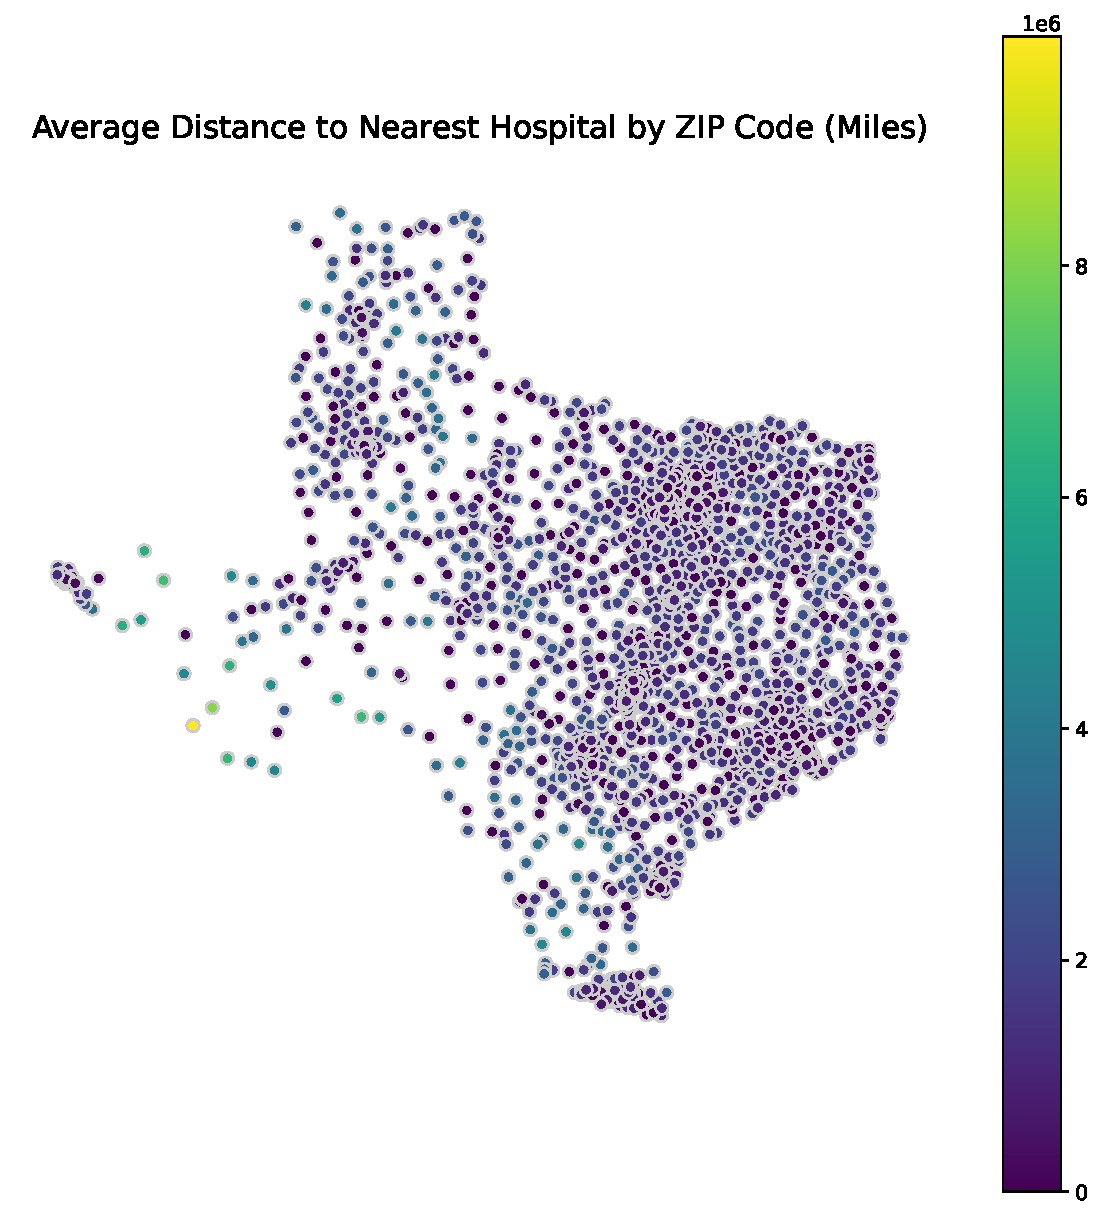
\includegraphics{pset4_ANSWERS_files/figure-pdf/cell-23-output-1.pdf}

\subsection{Effects of closures on access in Texas (15
pts)}\label{effects-of-closures-on-access-in-texas-15-pts}

\begin{enumerate}
\def\labelenumi{\arabic{enumi}.}
\tightlist
\item
\end{enumerate}

\begin{Shaded}
\begin{Highlighting}[]
\CommentTok{\# Define Texas ZIP code prefixes}
\NormalTok{zip\_texas\_prefixes }\OperatorTok{=}\NormalTok{ [}\StringTok{\textquotesingle{}75\textquotesingle{}}\NormalTok{, }\StringTok{\textquotesingle{}76\textquotesingle{}}\NormalTok{, }\StringTok{\textquotesingle{}77\textquotesingle{}}\NormalTok{, }\StringTok{\textquotesingle{}78\textquotesingle{}}\NormalTok{, }\StringTok{\textquotesingle{}79\textquotesingle{}}\NormalTok{, }\StringTok{\textquotesingle{}733\textquotesingle{}}\NormalTok{, }\StringTok{\textquotesingle{}885\textquotesingle{}}\NormalTok{]}

\CommentTok{\# Filter for closures in Texas between 2016{-}2019 based on ZIP code prefixes}
\NormalTok{texas\_closures\_2016\_2019 }\OperatorTok{=}\NormalTok{ confirmed\_closures\_df[}
\NormalTok{    (confirmed\_closures\_df[}\StringTok{\textquotesingle{}ZIP\_CD\textquotesingle{}}\NormalTok{].astype(}\BuiltInTok{str}\NormalTok{).}\BuiltInTok{str}\NormalTok{.startswith(}\BuiltInTok{tuple}\NormalTok{(zip\_texas\_prefixes))) }\OperatorTok{\&}
\NormalTok{    (confirmed\_closures\_df[}\StringTok{\textquotesingle{}Suspected Closure Year\textquotesingle{}}\NormalTok{] }\OperatorTok{\textgreater{}=} \DecValTok{2016}\NormalTok{) }\OperatorTok{\&}
\NormalTok{    (confirmed\_closures\_df[}\StringTok{\textquotesingle{}Suspected Closure Year\textquotesingle{}}\NormalTok{] }\OperatorTok{\textless{}=} \DecValTok{2019}\NormalTok{)}
\NormalTok{]}

\CommentTok{\# Count closures by ZIP code}
\NormalTok{closures\_by\_zip }\OperatorTok{=}\NormalTok{ texas\_closures\_2016\_2019[}\StringTok{\textquotesingle{}ZIP\_CD\textquotesingle{}}\NormalTok{].value\_counts(}
\NormalTok{).reset\_index()}
\NormalTok{closures\_by\_zip.columns }\OperatorTok{=}\NormalTok{ [}\StringTok{\textquotesingle{}ZIP\_CD\textquotesingle{}}\NormalTok{, }\StringTok{\textquotesingle{}Number of Closures\textquotesingle{}}\NormalTok{]}

\CommentTok{\# Display the table}
\BuiltInTok{print}\NormalTok{(}\StringTok{"Number of Hospital Closures by ZIP Code in Texas (2016{-}2019):"}\NormalTok{)}
\BuiltInTok{print}\NormalTok{(closures\_by\_zip.to\_string(index}\OperatorTok{=}\VariableTok{False}\NormalTok{))}

\CommentTok{\# Get the list of directly affected ZIP codes}
\NormalTok{affected\_zip\_codes }\OperatorTok{=}\NormalTok{ closures\_by\_zip[}\StringTok{\textquotesingle{}ZIP\_CD\textquotesingle{}}\NormalTok{].tolist()}

\BuiltInTok{print}\NormalTok{(}\SpecialStringTok{f"}\CharTok{\textbackslash{}n}\SpecialStringTok{Directly affected ZIP codes: }\SpecialCharTok{\{}\NormalTok{affected\_zip\_codes}\SpecialCharTok{\}}\SpecialStringTok{"}\NormalTok{)}
\BuiltInTok{print}\NormalTok{(}\SpecialStringTok{f"Total number of affected ZIP codes: }\SpecialCharTok{\{}\BuiltInTok{len}\NormalTok{(affected\_zip\_codes)}\SpecialCharTok{\}}\SpecialStringTok{"}\NormalTok{)}

\CommentTok{\# Calculate total number of closures}
\NormalTok{total\_closures }\OperatorTok{=}\NormalTok{ closures\_by\_zip[}\StringTok{\textquotesingle{}Number of Closures\textquotesingle{}}\NormalTok{].}\BuiltInTok{sum}\NormalTok{()}
\BuiltInTok{print}\NormalTok{(}\SpecialStringTok{f"Total number of hospital closures: }\SpecialCharTok{\{}\NormalTok{total\_closures}\SpecialCharTok{\}}\SpecialStringTok{"}\NormalTok{)}
\end{Highlighting}
\end{Shaded}

\begin{verbatim}
Number of Hospital Closures by ZIP Code in Texas (2016-2019):
 ZIP_CD  Number of Closures
76502.0                   1
75601.0                   1
75087.0                   1
76520.0                   1
78017.0                   1
78613.0                   1
75051.0                   1
78734.0                   1
77035.0                   1
77429.0                   1
75235.0                   1
79902.0                   1
75390.0                   1
76531.0                   1
75862.0                   1
79529.0                   1
77065.0                   1
78834.0                   1
78336.0                   1
75835.0                   1
75662.0                   1
79553.0                   1
78061.0                   1
75042.0                   1
79520.0                   1
76645.0                   1
79735.0                   1
75140.0                   1

Directly affected ZIP codes: [76502.0, 75601.0, 75087.0, 76520.0, 78017.0, 78613.0, 75051.0, 78734.0, 77035.0, 77429.0, 75235.0, 79902.0, 75390.0, 76531.0, 75862.0, 79529.0, 77065.0, 78834.0, 78336.0, 75835.0, 75662.0, 79553.0, 78061.0, 75042.0, 79520.0, 76645.0, 79735.0, 75140.0]
Total number of affected ZIP codes: 28
Total number of hospital closures: 28
\end{verbatim}

\begin{enumerate}
\def\labelenumi{\arabic{enumi}.}
\setcounter{enumi}{1}
\tightlist
\item
\end{enumerate}

\begin{Shaded}
\begin{Highlighting}[]
\CommentTok{\# Define Texas ZIP code prefixes (already defined in your previous code)}
\NormalTok{zip\_texas\_prefixes }\OperatorTok{=}\NormalTok{ [}\StringTok{\textquotesingle{}75\textquotesingle{}}\NormalTok{, }\StringTok{\textquotesingle{}76\textquotesingle{}}\NormalTok{, }\StringTok{\textquotesingle{}77\textquotesingle{}}\NormalTok{, }\StringTok{\textquotesingle{}78\textquotesingle{}}\NormalTok{, }\StringTok{\textquotesingle{}79\textquotesingle{}}\NormalTok{, }\StringTok{\textquotesingle{}733\textquotesingle{}}\NormalTok{, }\StringTok{\textquotesingle{}885\textquotesingle{}}\NormalTok{]}

\CommentTok{\# Filter for Texas ZIP codes based on their prefixes (reuse zip\_restrict)}
\NormalTok{zip\_restrict[}\StringTok{\textquotesingle{}ZIP\textquotesingle{}}\NormalTok{] }\OperatorTok{=}\NormalTok{ zip\_restrict[}\StringTok{\textquotesingle{}ZCTA5\textquotesingle{}}\NormalTok{].astype(}\BuiltInTok{str}\NormalTok{)}
\NormalTok{zip\_texas }\OperatorTok{=}\NormalTok{ zip\_restrict[zip\_restrict[}\StringTok{\textquotesingle{}ZIP\textquotesingle{}}\NormalTok{].}\BuiltInTok{str}\NormalTok{.startswith(}
    \BuiltInTok{tuple}\NormalTok{(zip\_texas\_prefixes))]}

\CommentTok{\# Ensure closures\_by\_zip has consistent formatting (convert to string and remove decimal points)}
\NormalTok{closures\_by\_zip[}\StringTok{\textquotesingle{}ZIP\_CD\textquotesingle{}}\NormalTok{] }\OperatorTok{=}\NormalTok{ closures\_by\_zip[}\StringTok{\textquotesingle{}ZIP\_CD\textquotesingle{}}\NormalTok{].fillna(}
    \DecValTok{0}\NormalTok{).astype(}\BuiltInTok{int}\NormalTok{).astype(}\BuiltInTok{str}\NormalTok{)}

\CommentTok{\# Debugging: Print sample data from both datasets to check for matching ZIP codes}
\BuiltInTok{print}\NormalTok{(}\StringTok{"Sample of closures\_by\_zip:"}\NormalTok{)}
\BuiltInTok{print}\NormalTok{(closures\_by\_zip.head())}

\BuiltInTok{print}\NormalTok{(}\StringTok{"}\CharTok{\textbackslash{}n}\StringTok{Sample of zip\_texas:"}\NormalTok{)}
\BuiltInTok{print}\NormalTok{(zip\_texas[[}\StringTok{\textquotesingle{}ZCTA5\textquotesingle{}}\NormalTok{, }\StringTok{\textquotesingle{}ZIP\textquotesingle{}}\NormalTok{]].head())}

\CommentTok{\# Merge the closure data with the shapefile data for Texas ZIP codes}
\NormalTok{zip\_texas\_closure\_map }\OperatorTok{=}\NormalTok{ zip\_texas.merge(}
\NormalTok{    closures\_by\_zip, left\_on}\OperatorTok{=}\StringTok{\textquotesingle{}ZIP\textquotesingle{}}\NormalTok{, right\_on}\OperatorTok{=}\StringTok{\textquotesingle{}ZIP\_CD\textquotesingle{}}\NormalTok{, how}\OperatorTok{=}\StringTok{\textquotesingle{}left\textquotesingle{}}\NormalTok{)}

\CommentTok{\# Fill NaN values in \textquotesingle{}Number of Closures\textquotesingle{} with 0 (for ZIPs with no closures)}
\NormalTok{zip\_texas\_closure\_map[}\StringTok{\textquotesingle{}Number of Closures\textquotesingle{}}\NormalTok{] }\OperatorTok{=}\NormalTok{ zip\_texas\_closure\_map[}\StringTok{\textquotesingle{}Number of Closures\textquotesingle{}}\NormalTok{].fillna(}
    \DecValTok{0}\NormalTok{)}

\CommentTok{\# Debugging: Check if any closures were found after merging}
\BuiltInTok{print}\NormalTok{(}\StringTok{"}\CharTok{\textbackslash{}n}\StringTok{Sample of merged data (after filling NaNs):"}\NormalTok{)}
\BuiltInTok{print}\NormalTok{(zip\_texas\_closure\_map[[}\StringTok{\textquotesingle{}ZIP\textquotesingle{}}\NormalTok{, }\StringTok{\textquotesingle{}Number of Closures\textquotesingle{}}\NormalTok{]].head())}
\end{Highlighting}
\end{Shaded}

\begin{verbatim}
Sample of closures_by_zip:
  ZIP_CD  Number of Closures
0  76502                   1
1  75601                   1
2  75087                   1
3  76520                   1
4  78017                   1

Sample of zip_texas:
      ZCTA5    ZIP
9207  78624  78624
9208  78626  78626
9209  78628  78628
9210  78631  78631
9211  78632  78632

Sample of merged data (after filling NaNs):
     ZIP  Number of Closures
0  78624                 0.0
1  78626                 0.0
2  78628                 0.0
3  78631                 0.0
4  78632                 0.0
\end{verbatim}

\begin{Shaded}
\begin{Highlighting}[]
\CommentTok{\# Plot a choropleth map of the number of closures by ZIP code in Texas}
\NormalTok{fig, ax }\OperatorTok{=}\NormalTok{ plt.subplots(}\DecValTok{1}\NormalTok{, }\DecValTok{1}\NormalTok{, figsize}\OperatorTok{=}\NormalTok{(}\DecValTok{10}\NormalTok{, }\DecValTok{10}\NormalTok{))}
\NormalTok{zip\_texas\_closure\_map.plot(column}\OperatorTok{=}\StringTok{\textquotesingle{}Number of Closures\textquotesingle{}}\NormalTok{, cmap}\OperatorTok{=}\StringTok{\textquotesingle{}Blues\textquotesingle{}}\NormalTok{,}
\NormalTok{                           linewidth}\OperatorTok{=}\FloatTok{0.8}\NormalTok{, ax}\OperatorTok{=}\NormalTok{ax, edgecolor}\OperatorTok{=}\StringTok{\textquotesingle{}0.8\textquotesingle{}}\NormalTok{, legend}\OperatorTok{=}\VariableTok{True}\NormalTok{)}

\NormalTok{plt.title(}\StringTok{\textquotesingle{}Texas ZIP Codes Affected by Hospital Closures (2016{-}2019)\textquotesingle{}}\NormalTok{, fontsize}\OperatorTok{=}\DecValTok{15}\NormalTok{)}
\NormalTok{plt.axis(}\StringTok{\textquotesingle{}off\textquotesingle{}}\NormalTok{)  }\CommentTok{\# Turn off axis}

\NormalTok{plt.show()}

\CommentTok{\# Count how many unique ZIP codes were directly affected by at least one closure}
\NormalTok{affected\_zip\_codes\_count }\OperatorTok{=}\NormalTok{ zip\_texas\_closure\_map[zip\_texas\_closure\_map[}\StringTok{\textquotesingle{}Number of Closures\textquotesingle{}}\NormalTok{] }\OperatorTok{\textgreater{}} \DecValTok{0}\NormalTok{][}\StringTok{\textquotesingle{}ZIP\textquotesingle{}}\NormalTok{].nunique(}
\NormalTok{)}
\BuiltInTok{print}\NormalTok{(}
    \SpecialStringTok{f"Total number of directly affected ZIP codes in Texas: }\SpecialCharTok{\{}\NormalTok{affected\_zip\_codes\_count}\SpecialCharTok{\}}\SpecialStringTok{"}\NormalTok{)}
\end{Highlighting}
\end{Shaded}

\includegraphics{pset4_ANSWERS_files/figure-pdf/cell-26-output-1.pdf}

\begin{verbatim}
Total number of directly affected ZIP codes in Texas: 28
\end{verbatim}

\begin{enumerate}
\def\labelenumi{\arabic{enumi}.}
\setcounter{enumi}{2}
\tightlist
\item
\end{enumerate}

\begin{Shaded}
\begin{Highlighting}[]
\NormalTok{directly\_affected\_zip\_gdf }\OperatorTok{=}\NormalTok{ zip\_texas\_closure\_map[zip\_texas\_closure\_map[}\StringTok{\textquotesingle{}Number of Closures\textquotesingle{}}\NormalTok{] }\OperatorTok{\textgreater{}} \DecValTok{0}\NormalTok{]}
\end{Highlighting}
\end{Shaded}

\begin{Shaded}
\begin{Highlighting}[]
\CommentTok{\# Adding uffer}
\NormalTok{buffered\_zips }\OperatorTok{=}\NormalTok{ directly\_affected\_zip\_gdf.copy()}
\NormalTok{buffered\_zips[}\StringTok{\textquotesingle{}geometry\textquotesingle{}}\NormalTok{] }\OperatorTok{=}\NormalTok{ buffered\_zips.geometry.}\BuiltInTok{buffer}\NormalTok{(}\FloatTok{16093.4}\NormalTok{)}
\end{Highlighting}
\end{Shaded}

\begin{Shaded}
\begin{Highlighting}[]
\CommentTok{\# Merging}
\NormalTok{buffered\_zips\_minimal }\OperatorTok{=}\NormalTok{ buffered\_zips[[}\StringTok{\textquotesingle{}ZIP\textquotesingle{}}\NormalTok{, }\StringTok{\textquotesingle{}geometry\textquotesingle{}}\NormalTok{]]}
\NormalTok{indirectly\_affected\_zip\_gdf }\OperatorTok{=}\NormalTok{ gpd.sjoin(}
\NormalTok{    zip\_texas,}
\NormalTok{    buffered\_zips\_minimal,}
\NormalTok{    how}\OperatorTok{=}\StringTok{\textquotesingle{}inner\textquotesingle{}}\NormalTok{,}
\NormalTok{    predicate}\OperatorTok{=}\StringTok{\textquotesingle{}intersects\textquotesingle{}}
\NormalTok{)}

\CommentTok{\# Remove ZIP codes that were directly affected}
\NormalTok{indirectly\_affected\_zip\_gdf }\OperatorTok{=}\NormalTok{ indirectly\_affected\_zip\_gdf[}
    \OperatorTok{\textasciitilde{}}\NormalTok{indirectly\_affected\_zip\_gdf[}\StringTok{\textquotesingle{}ZCTA5\textquotesingle{}}\NormalTok{].isin(}
\NormalTok{        directly\_affected\_zip\_gdf[}\StringTok{\textquotesingle{}ZIP\textquotesingle{}}\NormalTok{])}
\NormalTok{]}

\CommentTok{\# Count the number of indirectly affected ZIP codes}
\NormalTok{num\_indirectly\_affected\_zips }\OperatorTok{=}\NormalTok{ indirectly\_affected\_zip\_gdf[}\StringTok{\textquotesingle{}ZCTA5\textquotesingle{}}\NormalTok{].nunique()}
\BuiltInTok{print}\NormalTok{(}
    \SpecialStringTok{f"Number of indirectly affected ZIP codes: }\SpecialCharTok{\{}\NormalTok{num\_indirectly\_affected\_zips}\SpecialCharTok{\}}\SpecialStringTok{"}\NormalTok{)}

\CommentTok{\# Display the first few rows of the result to verify}
\BuiltInTok{print}\NormalTok{(indirectly\_affected\_zip\_gdf[[}\StringTok{\textquotesingle{}ZCTA5\textquotesingle{}}\NormalTok{]].head())}

\CommentTok{\# Create a list of unique indirectly affected ZIP codes}
\NormalTok{indirectly\_affected\_zip\_list }\OperatorTok{=}\NormalTok{ indirectly\_affected\_zip\_gdf[}\StringTok{\textquotesingle{}ZCTA5\textquotesingle{}}\NormalTok{].unique(}
\NormalTok{).tolist()}
\BuiltInTok{print}\NormalTok{(}\SpecialStringTok{f"List of indirectly affected ZIP codes: }\SpecialCharTok{\{}\NormalTok{indirectly\_affected\_zip\_list}\SpecialCharTok{\}}\SpecialStringTok{"}\NormalTok{)}
\end{Highlighting}
\end{Shaded}

\begin{verbatim}
Number of indirectly affected ZIP codes: 1907
      ZCTA5
9207  78624
9207  78624
9207  78624
9207  78624
9207  78624
List of indirectly affected ZIP codes: ['78624', '78626', '78628', '78631', '78632', '78633', '78634', '78635', '78636', '78638', '78639', '78640', '78641', '78642', '78643', '78645', '78654', '78659', '78661', '78663', '78665', '78670', '78672', '78676', '78681', '78703', '78704', '78722', '78723', '78725', '78727', '78730', '78732', '78736', '78738', '78742', '78745', '78747', '78753', '78754', '78758', '78759', '78827', '78828', '78832', '78837', '78840', '78850', '78872', '78877', '78881', '78885', '78931', '78933', '78935', '78940', '78942', '78945', '78947', '78949', '78953', '78956', '78963', '79003', '79007', '79010', '79012', '79015', '75558', '75559', '75560', '75561', '75562', '75563', '75565', '75566', '75567', '75568', '75570', '75571', '75573', '75574', '75602', '75604', '75630', '75638', '75640', '75643', '75650', '75652', '75656', '75668', '75670', '75682', '75684', '75692', '75693', '75703', '75705', '75707', '75750', '75752', '75755', '75757', '75763', '75765', '75771', '75778', '75783', '75784', '75788', '75791', '75801', '75831', '75839', '75845', '75849', '75852', '75855', '75859', '75861', '75901', '75925', '75929', '75931', '75936', '75938', '75941', '75943', '75951', '75956', '75960', '75964', '75966', '79016', '79018', '79019', '79021', '79022', '79027', '79029', '79031', '79032', '79034', '79035', '79036', '79039', '79041', '79043', '79045', '79052', '79057', '79059', '79062', '79064', '79070', '79080', '79082', '79084', '79087', '79091', '79093', '79097', '79105', '79106', '79107', '79108', '79110', '79119', '79124', '79220', '79226', '79229', '79233', '79237', '79241', '79243', '79248', '79250', '79252', '79256', '79259', '79311', '79313', '79316', '79324', '79326', '79336', '79345', '79347', '79351', '79356', '79358', '79360', '79364', '79367', '79371', '79373', '79380', '79382', '79403', '79407', '75969', '75972', '75973', '75974', '75975', '75976', '75977', '75980', '76001', '76002', '76006', '76008', '76009', '76010', '76012', '76014', '76016', '76018', '76023', '76028', '76033', '76040', '76043', '76048', '76050', '76052', '76055', '76060', '76061', '76064', '76066', '76070', '76073', '76085', '76087', '76092', '76103', '76107', '76110', '76111', '76114', '76117', '76119', '76123', '76127', '76133', '76137', '76155', '76164', '76179', '76201', '76205', '76209', '76225', '76227', '76230', '76238', '76245', '76248', '76250', '76255', '76258', '76261', '76263', '76266', '76270', '76272', '76301', '76305', '76351', '79415', '79416', '79424', '79501', '79502', '79503', '79504', '79505', '79506', '79510', '79511', '79512', '79517', '79518', '79519', '79521', '79527', '79532', '79536', '79539', '79541', '79544', '79546', '79548', '79561', '79563', '79566', '79601', '79605', '79701', '79705', '79718', '79719', '79731', '79734', '79738', '79742', '79744', '79748', '79752', '79759', '79762', '79764', '79766', '79777', '79780', '79782', '79785', '79789', '79831', '79835', '79837', '79842', '79847', '79851', '79853', '79904', '79905', '79907', '79912', '79922', '79924', '79925', '79934', '79936', '76354', '76357', '76360', '76363', '76364', '76365', '76367', '76370', '76371', '76372', '76374', '76377', '76379', '76380', '76384', '76388', '76424', '76426', '76431', '76437', '76443', '76445', '76448', '76452', '76454', '76457', '76459', '76462', '76464', '76470', '76475', '76481', '76486', '76491', '76501', '76504', '76513', '76519', '76522', '76524', '76527', '76530', '76539', '76542', '76544', '76550', '76556', '76559', '76565', '76567', '76570', '76574', '76578', '76624', '76626', '76627', '76629', '76631', '76633', '76636', '76638', '76640', '76642', '76649', '76655', '76656', '76660', '76664', '76666', '76670', '76671', '76673', '76676', '76678', '76679', '76680', '76681', '76682', '76685', '76687', '76689', '76690', '76691', '76692', '76705', '76706', '76708', '76712', '76801', '76820', '76823', '76828', '76832', '76837', '76842', '76845', '76849', '76854', '76857', '76859', '76865', '76870', '76872', '76878', '76882', '76885', '76890', '76903', '76905', '76930', '76934', '76936', '76939', '76941', '76949', '76955', '76958', '77003', '77007', '77011', '77012', '77013', '77014', '77017', '77019', '77022', '77024', '77030', '77031', '77032', '77037', '77041', '77043', '77045', '77048', '77053', '77054', '77055', '77060', '77061', '77063', '77064', '77066', '77068', '77069', '77070', '77071', '77072', '77073', '77074', '77075', '77077', '77078', '77079', '77081', '77086', '77088', '77090', '77092', '77094', '77099', '77301', '77304', '77316', '77326', '77328', '77336', '77340', '77345', '77350', '77354', '77356', '77358', '77362', '77364', '77367', '77371', '77373', '77377', '77379', '77382', '77385', '77388', '77396', '77407', '77414', '77418', '77420', '77423', '77428', '77432', '77437', '77441', '77444', '77449', '77450', '77455', '77456', '77458', '77461', '77465', '77467', '77469', '77475', '77477', '77480', '77481', '77482', '77484', '77485', '77486', '77488', '77489', '77493', '77494', '77498', '77502', '77503', '77505', '77511', '77515', '77519', '77521', '77530', '77532', '77534', '77536', '77539', '77546', '77550', '77554', '77562', '77566', '77571', '77575', '77580', '77583', '77585', '77590', '77597', '77611', '77613', '77615', '77622', '77625', '77629', '77640', '77642', '77655', '77657', '77660', '77662', '77703', '77705', '77707', '77803', '77808', '77831', '77835', '77840', '77853', '77856', '77859', '77865', '77868', '77872', '77876', '77904', '77950', '77954', '77960', '77962', '77968', '77970', '77973', '77975', '75006', '75009', '75013', '75020', '75022', '75024', '75032', '75039', '75041', '75043', '75050', '75052', '75056', '75058', '75061', '75063', '75068', '75070', '75074', '75078', '75082', '75090', '75093', '75098', '75103', '75105', '75110', '75115', '75119', '75125', '75127', '75142', '75144', '77976', '77978', '77979', '77982', '77983', '77984', '77990', '77993', '77994', '77995', '78002', '78003', '78004', '78007', '78009', '78011', '78013', '78015', '78022', '78024', '78026', '78039', '78043', '78045', '78050', '78056', '78058', '78064', '78066', '78069', '78071', '78073', '78104', '78108', '78112', '78116', '78118', '78121', '78123', '78125', '78132', '78145', '78146', '78148', '78154', '78159', '78161', '78163', '78204', '78205', '78207', '78209', '78211', '78213', '78216', '78218', '78220', '78224', '78227', '78229', '78231', '78233', '78236', '78238', '78240', '78244', '78245', '75147', '75148', '75149', '75152', '75153', '75154', '75155', '75156', '75158', '75159', '75160', '75163', '75165', '75166', '75167', '75169', '75173', '75181', '75189', '75203', '75206', '75207', '75209', '75211', '75217', '75219', '75223', '75227', '75228', '75230', '75232', '75234', '75236', '75240', '75243', '75252', '75254', '75287', '75401', '75407', '75410', '75414', '75415', '75417', '75420', '75422', '75431', '75433', '75436', '75438', '75441', '75446', '75448', '75450', '75453', '75455', '75459', '75468', '75470', '75474', '75476', '75478', '75481', '75486', '75488', '75490', '75493', '75495', '75503', '75551', '78249', '78250', '78251', '78253', '78254', '78255', '78256', '78257', '78258', '78259', '78260', '78263', '78264', '78266', '78332', '78341', '78343', '78344', '78353', '78355', '78358', '78362', '78370', '78372', '78374', '78376', '78380', '78383', '78385', '78390', '78393', '78402', '78405', '78408', '78414', '78417', '78418', '78503', '78516', '78521', '78536', '78537', '78539', '78543', '78548', '78550', '78559', '78562', '78564', '78566', '78569', '78573', '78575', '78577', '78579', '78582', '78584', '78591', '78592', '78595', '78596', '78598', '78606', '78608', '78610', '78614', '78619', '78621', '75569', '75603', '75605', '75631', '75633', '75639', '75641', '75642', '75644', '75647', '75651', '78644', '78648', '78652', '78653', '78655', '78657', '78660', '78662', '78664', '78666', '78669', '78671', '78675', '78677', '78701', '75654', '75657', '75661', '75667', '75669', '75672', '75681', '75683', '75686', '75691', '75701', '75702', '75704', '75706', '75708', '75709', '75751', '75754', '75756', '75758', '75759', '75762', '75764', '75766', '75770', '75773', '75779', '75780', '75785', '75789', '75790', '75792', '75803', '75832', '75833', '75838', '75840', '75844', '75846', '78702', '78705', '78712', '78719', '78721', '78724', '78726', '78728', '78729', '78731', '78733', '78735', '78737', '78739', '75848', '75850', '75851', '75853', '75856', '75858', '75860', '75904', '75926', '75928', '75930', '75932', '75934', '75935', '75937', '75939', '75942', '75944', '75946', '75949', '75954', '75959', '75961', '75962', '75965', '78741', '78744', '78746', '78748', '78750', '78751', '78752', '78756', '79025', '79033', '79040', '79042', '79044', '79046', '79051', '79053', '79056', '79058', '79061', '79063', '79065', '79068', '79072', '79079', '79081', '79083', '79085', '79086', '79088', '79092', '79094', '78757', '78801', '78802', '78829', '78830', '78833', '78836', '78838', '78839', '78843', '78851', '78860', '78861', '78871', '78873', '78879', '78880', '78883', '78884', '78886', '78932', '78934', '78938', '78941', '78943', '78944', '78946', '78948', '78950', '79096', '79406', '78951', '78954', '78957', '78962', '79001', '79005', '79009', '79011', '79013', '79014', '79098', '79101', '79102', '79103', '79104', '79109', '79111', '79118', '79121', '79201', '79225', '79227', '79230', '79231', '79234', '79236', '79239', '79240', '79244', '79245', '79247', '79251', '79255', '79257', '79258', '79261', '79312', '79314', '79322', '79323', '79325', '79329', '79331', '79339', '79342', '79344', '79346', '79350', '79353', '79355', '79357', '79359', '79363', '79366', '79369', '79370', '79372', '79376', '79377', '79379', '79381', '79401', '79404', '79525', '79526', '79528', '79530', '79533', '79535', '79537', '79538', '79540', '79543', '79545', '79547', '79549', '79556', '79560', '79562', '79565', '79567', '79602', '79603', '79607', '79699', '79703', '79706', '79713', '79714', '79720', '79730', '79733', '79739', '79741', '79743', '79745', '79749', '79754', '79755', '79758', '79761', '79763', '79765', '79770', '79772', '79778', '79781', '76596', '76597', '76598', '76599', '76623', '76628', '76630', '76632', '76634', '76635', '76637', '76639', '76641', '77050', '77051', '77056', '77057', '77059', '79414', '79783', '76643', '77076', '77080', '77082', '77084', '77085', '77087', '77089', '77091', '77093', '77095', '77098', '77201', '77303', '77306', '77318', '77320', '77327', '77331', '77335', '77338', '77339', '77342', '77346', '77351', '77355', '77357', '77359', '77360', '77363', '77365', '77368', '77369', '77372', '77374', '77378', '77380', '77381', '77384', '77386', '77389', '77401', '77406', '77412', '77415', '77417', '77419', '77422', '77426', '77430', '77433', '77435', '77977', '77987', '77988', '78005', '78006', '78008', '78010', '78012', '78014', '78016', '78019', '78021', '78023', '78025', '78027', '78029', '78040', '78041', '78044', '78046', '78052', '78055', '78057', '78059', '77096', '77440', '77442', '77443', '77445', '77447', '77448', '77451', '77453', '77454', '77457', '77459', '77376', '77506', '77507', '77514', '77517', '77518', '77520', '77523', '77531', '77533', '77535', '77538', '77541', '77545', '77547', '77551', '77560', '77561', '77563', '77565', '77568', '77573', '77577', '77578', '77436', '78060', '78063', '78065', '78067', '78070', '78072', '78075', '78076', '78102', '78107', '78109', '78113', '78114', '78117', '78119', '78122', '78124', '78130', '78133', '78140', '78142', '78143', '77062', '77460', '77464', '77466', '77468', '77470', '77473', '77474', '77476', '77478', '77479', '77581', '77584', '77586', '77587', '77591', '77598', '77612', '77614', '77616', '77617', '77619', '77624', '77627', '77630', '77632', '77650', '77651', '77656', '77659', '77661', '77663', '78144', '78147', '78150', '78152', '78155', '78160', '78162', '78164', '78201', '78202', '78203', '78208', '78210', '78212', '78214', '77664', '77701', '77702', '77706', '77708', '77801', '77802', '77807', '77830', '77833', '77836', '77837', '77845', '77855', '77857', '77861', '77864', '77867', '77871', '77873', '77878', '77880', '77901', '77905', '77951', '77957', '78215', '78217', '78219', '78221', '78223', '78225', '78226', '78228', '78230', '78232', '78234', '78235', '78237', '78239', '78242', '77961', '77963', '77964', '77969', '77971', '77974', '78243', '75226', '75229', '75231', '75233', '75237', '75238', '75241', '75244', '75246', '75249', '75251', '75253', '78247', '78248', '75157', '75164', '75172', '75180', '75182', '75201', '75202', '75001', '75002', '75007', '75010', '75019', '75021', '75023', '75025', '75028', '75034', '75204', '75205', '75208', '75210', '75212', '75214', '75216', '75218', '75220', '75224', '75225', '75038', '75040', '75044', '75048', '75054', '75057', '75060', '75062', '75065', '75067', '75069', '75071', '75075', '75077', '75080', '75081', '75089', '75092', '75094', '75101', '75102', '75104', '75109', '75114', '75116', '75117', '75124', '75126', '75132', '75135', '75137', '75141', '75143', '75146', '79788', '79821', '79830', '79834', '79836', '79838', '79839', '79843', '79846', '79848', '79849', '79852', '79854', '79855', '79901', '79903', '79906', '79908', '76648', '76650', '76651', '76653', '76654', '76657', '76661', '76665', '76667', '76693', '76701', '75978', '76011', '76013', '76015', '76017', '76020', '76021', '79911', '79915', '79916', '79920', '79927', '79930', '79932', '79935', '79938', '76704', '76707', '76710', '76711', '76798', '76802', '76821', '76824', '76827', '76831', '76834', '76836', '76841', '76844', '76848', '76852', '76853', '76856', '76858', '76861', '76864', '76866', '76869', '76871', '76873', '76875', '76877', '76884', '76887', '76888', '76031', '76034', '76036', '76039', '76041', '76044', '76049', '76051', '76053', '76054', '76058', '76059', '76063', '76065', '76067', '76071', '76077', '76078', '76084', '76086', '76088', '76901', '76904', '76908', '76932', '76933', '76935', '76937', '76940', '76943', '76945', '76950', '76953', '76957', '77002', '77004', '76022', '76093', '76102', '76104', '76106', '76108', '76109', '76112', '76115', '76116', '76118', '76120', '76126', '76129', '76132', '76134', '76135', '76140', '76148', '76177', '76180', '76182', '76207', '76208', '76210', '77005', '77006', '77008', '77009', '77010', '77015', '76226', '76228', '76233', '76234', '76239', '76244', '76247', '76249', '76251', '76252', '76253', '76259', '76262', '76264', '76265', '76268', '76271', '76273', '76302', '76306', '76308', '76373', '76389', '76401', '76402', '76427', '76430', '76432', '76433', '76436', '76442', '76444', '76446', '76449', '76450', '76453', '76455', '76458', '76460', '76463', '76466', '76469', '76471', '76474', '76476', '76483', '77016', '77018', '77020', '77021', '77023', '77025', '77026', '76309', '76311', '79410', '79411', '79412', '79413', '76484', '76487', '76490', '76508', '76511', '76518', '76523', '76525', '76528', '76534', '76538', '76541', '76543', '76548', '76549', '76554', '76557', '76561', '76566', '76569', '76571', '76573', '76577', '76579', '77027', '77028', '77033', '77034', '77036', '77038', '77040', '77042', '77044', '77046', '77047', '77049', '75270', '75402', '75409', '75411', '75412', '75413', '75416', '75418', '75421', '75423', '75426', '75428', '75432', '75435', '75437', '75439', '75440', '75442', '75447', '75449', '75451', '75452', '75454', '75457', '75460', '75462', '75469', '75471', '75473', '75475', '75477', '75479', '75480', '75482', '75487', '75489', '75491', '75492', '75494', '75496', '75501', '75550', '75554', '75555', '78330', '78335', '78338', '78339', '78340', '78342', '78349', '78351', '78352', '78357', '78361', '78363', '78369', '78371', '78373', '78375', '78377', '78379', '78382', '78384', '78387', '78389', '78391', '78401', '78404', '78406', '78407', '78409', '78411', '78413', '78415', '78416', '78419', '78501', '78504', '78520', '78526', '78535', '78538', '78541', '78542', '78545', '78549', '78552', '78359', '78558', '78560', '78561', '78563', '78565', '78567', '78570', '78572', '78574', '78576', '78578', '78580', '78583', '78585', '78588', '78589', '78590', '78593', '78594', '78597', '78602', '78605', '78607', '78609', '78611', '78612', '78615', '78616', '78618', '78620', '78622', '78623', '78656', '75645', '75933', '79078', '79343', '75968', '76105', '76310', '79423', '79707', '79928', '76435', '76621', '76862', '77039', '77302', '77446', '77504', '77665', '75088', '77991', '78141', '75150', '75247', '75497', '78252', '78410', '78617', '78852', '78629', '78650', '78717', '78749', '78870', '78959', '75556', '75572', '75760', '75847', '75948', '79024', '79054', '79095', '79235', '79330', '79378', '75979', '76035', '76082', '76131', '76240', '79508', '79534', '79606', '79756', '79845', '76366', '76429', '76472', '76537', '76622', '76652', '79942', '76686', '76825', '76874', '76951', '77029', '77058', '77067', '77083', '77334', '77375', '77434', '77471', '77483', '77510', '77564', '77623', '77713', '77879', '75035', '75076', '75134', '78001', '78028', '78101', '78151', '78222', '75161', '75215', '75248', '75424', '75472', '78261', '78368', '78412', '78557', '78586']
\end{verbatim}

\begin{Shaded}
\begin{Highlighting}[]
\ImportTok{import}\NormalTok{ matplotlib.pyplot }\ImportTok{as}\NormalTok{ plt}
\ImportTok{from}\NormalTok{ matplotlib.colors }\ImportTok{import}\NormalTok{ ListedColormap}
\ImportTok{from}\NormalTok{ matplotlib.patches }\ImportTok{import}\NormalTok{ Patch}
\end{Highlighting}
\end{Shaded}

\begin{Shaded}
\begin{Highlighting}[]
\CommentTok{\# 1. Define Texas ZIP code prefixes}
\NormalTok{zip\_texas\_prefixes }\OperatorTok{=}\NormalTok{ [}\StringTok{\textquotesingle{}75\textquotesingle{}}\NormalTok{, }\StringTok{\textquotesingle{}76\textquotesingle{}}\NormalTok{, }\StringTok{\textquotesingle{}77\textquotesingle{}}\NormalTok{, }\StringTok{\textquotesingle{}78\textquotesingle{}}\NormalTok{, }\StringTok{\textquotesingle{}79\textquotesingle{}}\NormalTok{, }\StringTok{\textquotesingle{}733\textquotesingle{}}\NormalTok{, }\StringTok{\textquotesingle{}885\textquotesingle{}}\NormalTok{]}

\CommentTok{\# 2. Filter for closures in Texas between 2016{-}2019 based on ZIP code prefixes}
\NormalTok{texas\_closures\_2016\_2019 }\OperatorTok{=}\NormalTok{ confirmed\_closures\_df[}
\NormalTok{    (confirmed\_closures\_df[}\StringTok{\textquotesingle{}ZIP\_CD\textquotesingle{}}\NormalTok{].astype(}\BuiltInTok{str}\NormalTok{).}\BuiltInTok{str}\NormalTok{.startswith(}\BuiltInTok{tuple}\NormalTok{(zip\_texas\_prefixes))) }\OperatorTok{\&}
\NormalTok{    (confirmed\_closures\_df[}\StringTok{\textquotesingle{}Suspected Closure Year\textquotesingle{}}\NormalTok{] }\OperatorTok{\textgreater{}=} \DecValTok{2016}\NormalTok{) }\OperatorTok{\&}
\NormalTok{    (confirmed\_closures\_df[}\StringTok{\textquotesingle{}Suspected Closure Year\textquotesingle{}}\NormalTok{] }\OperatorTok{\textless{}=} \DecValTok{2019}\NormalTok{)}
\NormalTok{]}

\CommentTok{\# 3. Count closures by ZIP code}
\NormalTok{closures\_by\_zip }\OperatorTok{=}\NormalTok{ texas\_closures\_2016\_2019[}\StringTok{\textquotesingle{}ZIP\_CD\textquotesingle{}}\NormalTok{].value\_counts(}
\NormalTok{).reset\_index()}
\NormalTok{closures\_by\_zip.columns }\OperatorTok{=}\NormalTok{ [}\StringTok{\textquotesingle{}ZIP\_CD\textquotesingle{}}\NormalTok{, }\StringTok{\textquotesingle{}Number of Closures\textquotesingle{}}\NormalTok{]}

\CommentTok{\# 4. Ensure closures\_by\_zip ZIP code column is string formatted for consistency}
\NormalTok{closures\_by\_zip[}\StringTok{\textquotesingle{}ZIP\_CD\textquotesingle{}}\NormalTok{] }\OperatorTok{=}\NormalTok{ closures\_by\_zip[}\StringTok{\textquotesingle{}ZIP\_CD\textquotesingle{}}\NormalTok{].fillna(}
    \DecValTok{0}\NormalTok{).astype(}\BuiltInTok{int}\NormalTok{).astype(}\BuiltInTok{str}\NormalTok{)}

\CommentTok{\# 5. Filter Texas ZIP codes based on prefixes and ensure they are strings}
\NormalTok{zip\_restrict[}\StringTok{\textquotesingle{}ZIP\textquotesingle{}}\NormalTok{] }\OperatorTok{=}\NormalTok{ zip\_restrict[}\StringTok{\textquotesingle{}ZCTA5\textquotesingle{}}\NormalTok{].astype(}\BuiltInTok{str}\NormalTok{)}
\NormalTok{zip\_texas }\OperatorTok{=}\NormalTok{ zip\_restrict[zip\_restrict[}\StringTok{\textquotesingle{}ZIP\textquotesingle{}}\NormalTok{].}\BuiltInTok{str}\NormalTok{.startswith(}
    \BuiltInTok{tuple}\NormalTok{(zip\_texas\_prefixes))]}

\CommentTok{\# 6. Merge closure data with Texas ZIP codes}
\NormalTok{zip\_texas\_closure\_map }\OperatorTok{=}\NormalTok{ zip\_texas.merge(}
\NormalTok{    closures\_by\_zip, left\_on}\OperatorTok{=}\StringTok{\textquotesingle{}ZIP\textquotesingle{}}\NormalTok{, right\_on}\OperatorTok{=}\StringTok{\textquotesingle{}ZIP\_CD\textquotesingle{}}\NormalTok{, how}\OperatorTok{=}\StringTok{\textquotesingle{}left\textquotesingle{}}
\NormalTok{)}

\CommentTok{\# 7. Fill NaN values in \textquotesingle{}Number of Closures\textquotesingle{} with 0 for ZIPs with no closures}
\NormalTok{zip\_texas\_closure\_map[}\StringTok{\textquotesingle{}Number of Closures\textquotesingle{}}\NormalTok{] }\OperatorTok{=}\NormalTok{ zip\_texas\_closure\_map[}\StringTok{\textquotesingle{}Number of Closures\textquotesingle{}}\NormalTok{].fillna(}
    \DecValTok{0}\NormalTok{)}

\CommentTok{\# 8. Convert to a projected CRS (meters) if necessary, and add a buffer}
\NormalTok{zip\_texas\_closure\_map }\OperatorTok{=}\NormalTok{ zip\_texas\_closure\_map.to\_crs(epsg}\OperatorTok{=}\DecValTok{3857}\NormalTok{)}
\NormalTok{buffered\_zips }\OperatorTok{=}\NormalTok{ zip\_texas\_closure\_map[zip\_texas\_closure\_map[}\StringTok{\textquotesingle{}Number of Closures\textquotesingle{}}\NormalTok{] }\OperatorTok{\textgreater{}} \DecValTok{0}\NormalTok{].copy(}
\NormalTok{)}
\NormalTok{buffered\_zips[}\StringTok{\textquotesingle{}geometry\textquotesingle{}}\NormalTok{] }\OperatorTok{=}\NormalTok{ buffered\_zips.geometry.}\BuiltInTok{buffer}\NormalTok{(}
    \FloatTok{16093.4}\NormalTok{)  }\CommentTok{\# 10{-}mile buffer}

\CommentTok{\# 9. Keep only the ZIP and geometry columns for the spatial join}
\NormalTok{buffered\_zips\_minimal }\OperatorTok{=}\NormalTok{ buffered\_zips[[}\StringTok{\textquotesingle{}ZIP\textquotesingle{}}\NormalTok{, }\StringTok{\textquotesingle{}geometry\textquotesingle{}}\NormalTok{]]}

\CommentTok{\# 10. Reproject the original Texas ZIP data to match CRS}
\NormalTok{zip\_texas }\OperatorTok{=}\NormalTok{ zip\_texas.to\_crs(epsg}\OperatorTok{=}\DecValTok{3857}\NormalTok{)}

\CommentTok{\# 11. Spatial join to find indirectly affected ZIP codes within the buffer}
\NormalTok{indirectly\_affected\_zip\_gdf }\OperatorTok{=}\NormalTok{ gpd.sjoin(}
\NormalTok{    zip\_texas,}
\NormalTok{    buffered\_zips\_minimal,}
\NormalTok{    how}\OperatorTok{=}\StringTok{\textquotesingle{}inner\textquotesingle{}}\NormalTok{,}
\NormalTok{    predicate}\OperatorTok{=}\StringTok{\textquotesingle{}intersects\textquotesingle{}}
\NormalTok{)}

\CommentTok{\# 12. Remove ZIP codes that were directly affected}
\NormalTok{indirectly\_affected\_zip\_gdf }\OperatorTok{=}\NormalTok{ indirectly\_affected\_zip\_gdf[}
    \OperatorTok{\textasciitilde{}}\NormalTok{indirectly\_affected\_zip\_gdf[}\StringTok{\textquotesingle{}ZCTA5\textquotesingle{}}\NormalTok{].isin(buffered\_zips[}\StringTok{\textquotesingle{}ZIP\textquotesingle{}}\NormalTok{])}
\NormalTok{]}

\CommentTok{\# 13. Add category columns for directly and indirectly affected ZIPs}
\NormalTok{zip\_texas\_closure\_map[}\StringTok{\textquotesingle{}Affected\_Category\textquotesingle{}}\NormalTok{] }\OperatorTok{=} \StringTok{\textquotesingle{}Not Affected\textquotesingle{}}
\NormalTok{zip\_texas\_closure\_map.loc[zip\_texas\_closure\_map[}\StringTok{\textquotesingle{}Number of Closures\textquotesingle{}}\NormalTok{]}
                          \OperatorTok{\textgreater{}} \DecValTok{0}\NormalTok{, }\StringTok{\textquotesingle{}Affected\_Category\textquotesingle{}}\NormalTok{] }\OperatorTok{=} \StringTok{\textquotesingle{}Directly Affected\textquotesingle{}}
\NormalTok{indirectly\_affected\_zips }\OperatorTok{=}\NormalTok{ indirectly\_affected\_zip\_gdf[}\StringTok{\textquotesingle{}ZCTA5\textquotesingle{}}\NormalTok{].unique()}
\NormalTok{zip\_texas\_closure\_map.loc[}
\NormalTok{    zip\_texas\_closure\_map[}\StringTok{\textquotesingle{}ZIP\textquotesingle{}}\NormalTok{].isin(indirectly\_affected\_zips),}
    \StringTok{\textquotesingle{}Affected\_Category\textquotesingle{}}
\NormalTok{] }\OperatorTok{=} \StringTok{\textquotesingle{}Indirectly Affected\textquotesingle{}}

\CommentTok{\# 14. Create a color map for the categories}
\CommentTok{\# Not Affected, Indirectly Affected, Directly Affected}
\NormalTok{colors }\OperatorTok{=}\NormalTok{ [}\StringTok{\textquotesingle{}\#E6E6E6\textquotesingle{}}\NormalTok{, }\StringTok{\textquotesingle{}\#FFA500\textquotesingle{}}\NormalTok{, }\StringTok{\textquotesingle{}\#FF0000\textquotesingle{}}\NormalTok{]}
\NormalTok{cmap }\OperatorTok{=}\NormalTok{ ListedColormap(colors)}

\CommentTok{\# 15. Map categories to integer codes for plotting}
\NormalTok{zip\_texas\_closure\_map[}\StringTok{\textquotesingle{}Category\_Code\textquotesingle{}}\NormalTok{] }\OperatorTok{=}\NormalTok{ zip\_texas\_closure\_map[}\StringTok{\textquotesingle{}Affected\_Category\textquotesingle{}}\NormalTok{].}\BuiltInTok{map}\NormalTok{(\{}
    \StringTok{\textquotesingle{}Not Affected\textquotesingle{}}\NormalTok{: }\DecValTok{0}\NormalTok{,}
    \StringTok{\textquotesingle{}Indirectly Affected\textquotesingle{}}\NormalTok{: }\DecValTok{1}\NormalTok{,}
    \StringTok{\textquotesingle{}Directly Affected\textquotesingle{}}\NormalTok{: }\DecValTok{2}
\NormalTok{\})}

\CommentTok{\# 16. Plot the data}
\NormalTok{fig, ax }\OperatorTok{=}\NormalTok{ plt.subplots(}\DecValTok{1}\NormalTok{, }\DecValTok{1}\NormalTok{, figsize}\OperatorTok{=}\NormalTok{(}\DecValTok{15}\NormalTok{, }\DecValTok{15}\NormalTok{))}
\NormalTok{zip\_texas\_closure\_map.plot(column}\OperatorTok{=}\StringTok{\textquotesingle{}Category\_Code\textquotesingle{}}\NormalTok{, cmap}\OperatorTok{=}\NormalTok{cmap, linewidth}\OperatorTok{=}\FloatTok{0.8}\NormalTok{,}
\NormalTok{                           edgecolor}\OperatorTok{=}\StringTok{\textquotesingle{}0.8\textquotesingle{}}\NormalTok{, ax}\OperatorTok{=}\NormalTok{ax, legend}\OperatorTok{=}\VariableTok{True}\NormalTok{)}

\CommentTok{\# Customize the legend}
\NormalTok{legend\_elements }\OperatorTok{=}\NormalTok{ [}
\NormalTok{    Patch(facecolor}\OperatorTok{=}\StringTok{\textquotesingle{}\#E6E6E6\textquotesingle{}}\NormalTok{, edgecolor}\OperatorTok{=}\StringTok{\textquotesingle{}black\textquotesingle{}}\NormalTok{, label}\OperatorTok{=}\StringTok{\textquotesingle{}Not Affected\textquotesingle{}}\NormalTok{),}
\NormalTok{    Patch(facecolor}\OperatorTok{=}\StringTok{\textquotesingle{}\#FFA500\textquotesingle{}}\NormalTok{, edgecolor}\OperatorTok{=}\StringTok{\textquotesingle{}black\textquotesingle{}}\NormalTok{, label}\OperatorTok{=}\StringTok{\textquotesingle{}Indirectly Affected\textquotesingle{}}\NormalTok{),}
\NormalTok{    Patch(facecolor}\OperatorTok{=}\StringTok{\textquotesingle{}\#FF0000\textquotesingle{}}\NormalTok{, edgecolor}\OperatorTok{=}\StringTok{\textquotesingle{}black\textquotesingle{}}\NormalTok{, label}\OperatorTok{=}\StringTok{\textquotesingle{}Directly Affected\textquotesingle{}}\NormalTok{)}
\NormalTok{]}
\NormalTok{ax.legend(handles}\OperatorTok{=}\NormalTok{legend\_elements,}
\NormalTok{          title}\OperatorTok{=}\StringTok{\textquotesingle{}Affected Categories\textquotesingle{}}\NormalTok{, loc}\OperatorTok{=}\StringTok{\textquotesingle{}lower right\textquotesingle{}}\NormalTok{)}

\CommentTok{\# Add title and remove axis}
\NormalTok{plt.title(}\StringTok{\textquotesingle{}Texas ZIP Codes Affected by Hospital Closures (2016{-}2019)\textquotesingle{}}\NormalTok{, fontsize}\OperatorTok{=}\DecValTok{16}\NormalTok{)}
\NormalTok{plt.axis(}\StringTok{\textquotesingle{}off\textquotesingle{}}\NormalTok{)}
\NormalTok{plt.show()}

\CommentTok{\# Summary statistics}
\BuiltInTok{print}\NormalTok{(}\StringTok{"Summary of Affected ZIP Codes:"}\NormalTok{)}
\BuiltInTok{print}\NormalTok{(zip\_texas\_closure\_map[}\StringTok{\textquotesingle{}Affected\_Category\textquotesingle{}}\NormalTok{].value\_counts())}
\end{Highlighting}
\end{Shaded}

\includegraphics{pset4_ANSWERS_files/figure-pdf/cell-31-output-1.pdf}

\begin{verbatim}
Summary of Affected ZIP Codes:
Affected_Category
Not Affected           1430
Indirectly Affected     477
Directly Affected        28
Name: count, dtype: int64
\end{verbatim}

\subsection{Reflecting on the exercise (10
pts)}\label{reflecting-on-the-exercise-10-pts}

(Partner 1) The method we use to identify closures is in fact imperfect.
For cases where hospitals rebranded, for example, there isn't actually a
merger or closure occurring, but the data will suggest that the old name
for the hosptial closed, essentially marking down a closure when there
was just a rebranding. Similarly, hospitals may delay in reporting
information about their active status due to simple human error.
Furthermore, there are hospitals that may only temporarily be closed,
and so adding them to the closure list is innaccurate given enough time.

I think one of the best solutions we can employ is to analyze data over
a longer period of time for more consistency. We may also consider
writing contingencies that allow us to find hospitals that have
rebranded. For example, if a hospital has location and provider
information identical to a previously closed hospital, perhaps there are
times where this is more accurate to flag as a rebrand rather than a
merger. It may be useful to cross-reference our data with our databases
that track whether a hospital can rebrand or whether their closure is
temporary~or~permanent.

(Partner 2) What our zipcode analysis lacks is nuance. While we analyze
which areas close and how this can affect other areas based on travel
time, we don't know exactly what kinds of hospitals are closing. Let's
say a relatively underutilized hospital closes but the most important
facilites are still open. Let's take another case where one of the most
visited facilities is the one to close. In our data, this difference
isn't detected, but in real life, that difference is crucial. In the
former case, relatively few individuals may be affected. In the latter,
this may be disastrous for nearby citizens' access to healthcare.
Perhaps some additional data analysis related to hospital type or
average patients received can help us further detect how impactful
closures within zipcodes will be.




\end{document}
